\section{Конструкторская часть}
\subsection{Формат входных данных}
В качестве входных данных выступает пользовательское описание какого-либо объекта. Оно должно соответствовать следующим требованиям:
\begin{enumerate}
	\item определение даётся полностью на русском языке;
	\item недопустимо использование аббревиатур, сокращений и т.д., все слова должны быть употреблены в полной форме;
	\item описание должно укладываться в 1-2 предложения;
	\item следует связно излагать свои мысли;
	\item допускается голосовой ввод, результат которого в дальнейшем будет преобразован в текстовый формат. \newline
\end{enumerate}

\subsection{Формат выходных данных}
Выходные данные представляются как множество терминов из выборки, каждому из которых поставлены в соответствие величина косинусного сходства и её промасштабированное значение, выраженное в процентах.

Если в ходе работы метода дополнительно привлекалась сеть синтаксических графов, то пользователю также предоставляется информация о количестве совпавших слов (в запросе пользователя и терминах сети) и процентное соотношение. 

Для интерпретации полученных значений косинусного сходства и количества совпавших слов используется функция softmax \cite{softmax} позволяющая перевести множество полученных значений в вектор процентов уверенности в том, что был описан соответствующий термин. \newline

\subsection{IDEF0}
Разрабатываемый метод состоит из нескольких этапов, которые представлены на рисунках \ref{fig20:image}-\ref{fig22:image}. Необходимо по изложению пользователя определить описываемый объект. 

\begin{figure}[h]
	\begin{center}
		{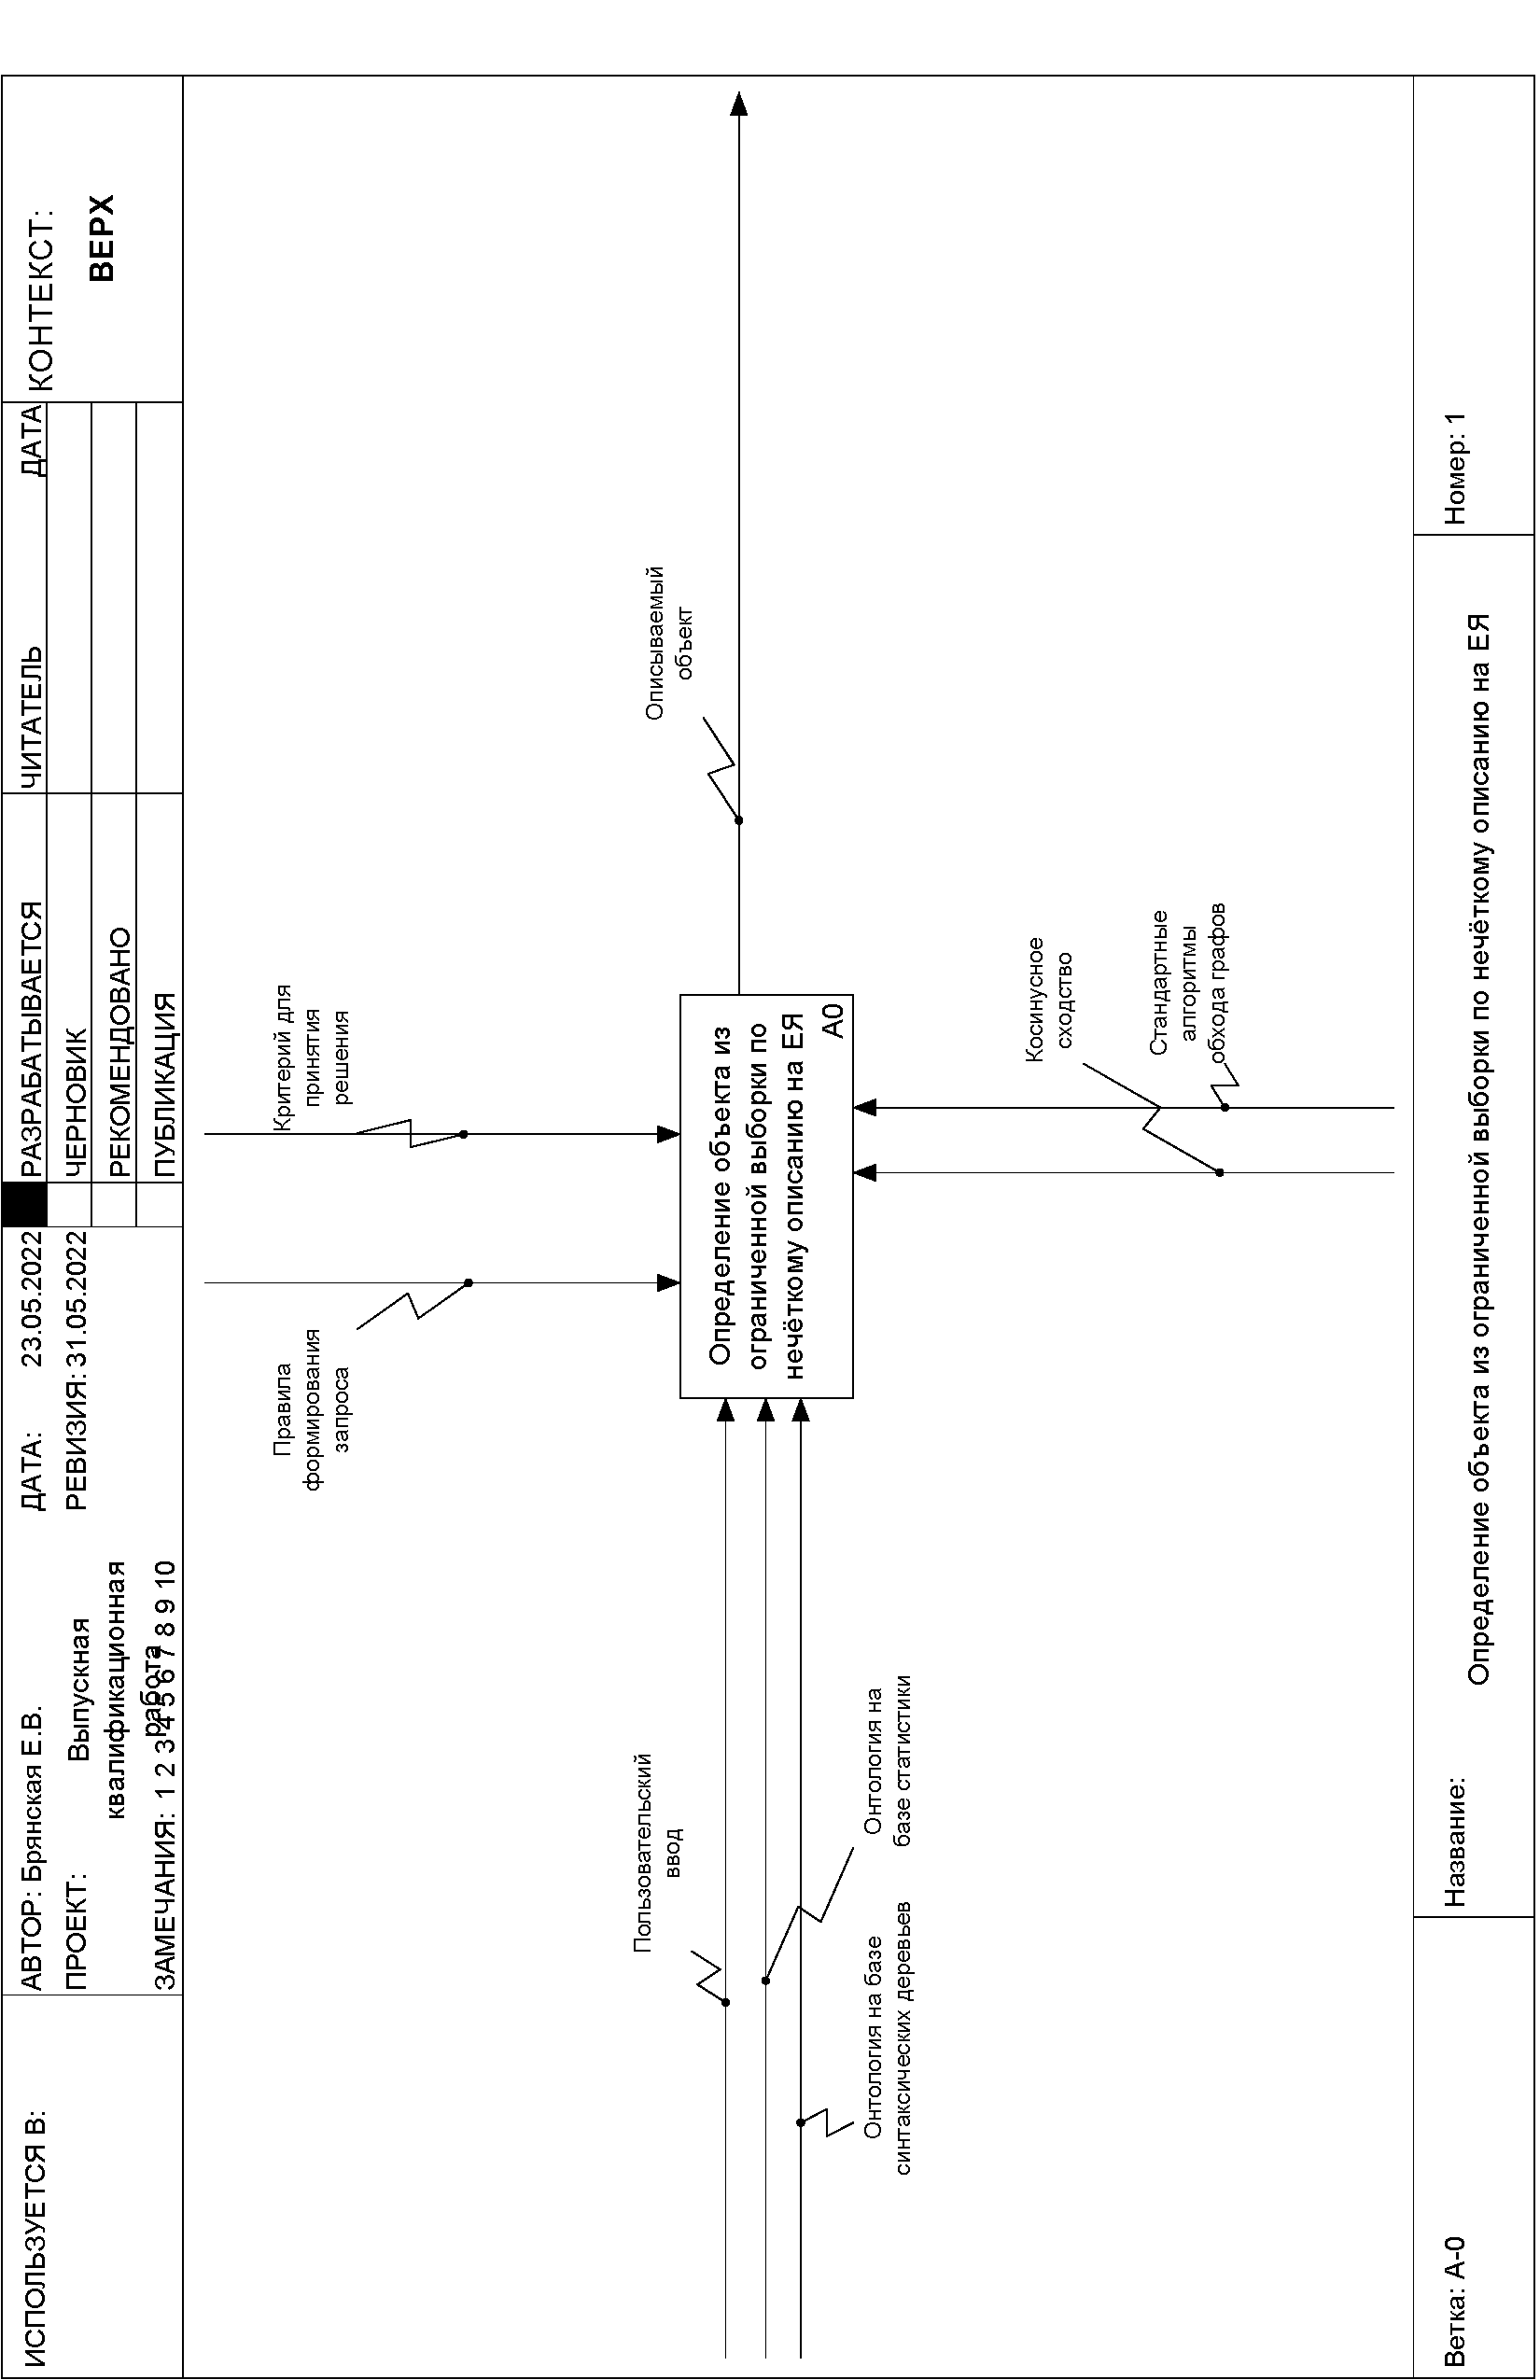
\includegraphics[scale = 0.39, angle=-90, page=1]{img/idef0/pdf/general.pdf}}
		\caption{Контекстная диаграмма основного метода.}
		\label{fig20:image}
	\end{center}
\end{figure}

Эта задача решается в несколько этапов: обработка запроса клиента, его преобразование, путём извлечения ключевых слов, сопоставление полученных данных с уже имеющимися онтологиями (сформированными на базе статистики и синтаксических графов), формирование промежуточного результата, и затем -- принятие решения о том, какой именно термин (один или несколько) наиболее подходит под это описание.
\begin{figure}[h]
	\begin{center}
		{\includegraphics[scale = 0.39, angle=-90, page=2]{img/idef0/pdf/general.pdf}}
		\caption{Декомпозиция основного метода.}
		\label{fig21:image}
	\end{center}
\end{figure}

\newpage

Алгоритм поиска нечётких дубликатов также состоит из нескольких этапов: сначала с помощью косинусного сходства определяются косинусные расстояния запроса пользователя и всех элементов статистической онтологии, затем, на основе полученных результатов принимается решение о том, нужно ли привлекать онтологию на основе синтаксических графов, чтобы увеличить точность распознавания термина. 

Если же результаты, полученные на первом этапе, удовлетворяют критерию принятия решения, то дальнейший анализ производиться не будет. 
\begin{figure}[h]
	\begin{center}
		{\includegraphics[scale = 0.39, angle=-90, page=3]{img/idef0/pdf/general.pdf}}
		\caption{Декомпозиция блока А3.}
		\label{fig22:image}
	\end{center}
\end{figure}

\newpage

В методе используется два подхода: статистический и на основе семантической сети, для каждого из них формируется онтология, процесс создания которой состоит из нескольких последовательных шагов.

Так формирование онтологии, в основе которой лежит статистические данные, представлено на рисунках \ref{fig23:image}-\ref{fig24:image}. 
\begin{figure}[h]
	\begin{center}
		{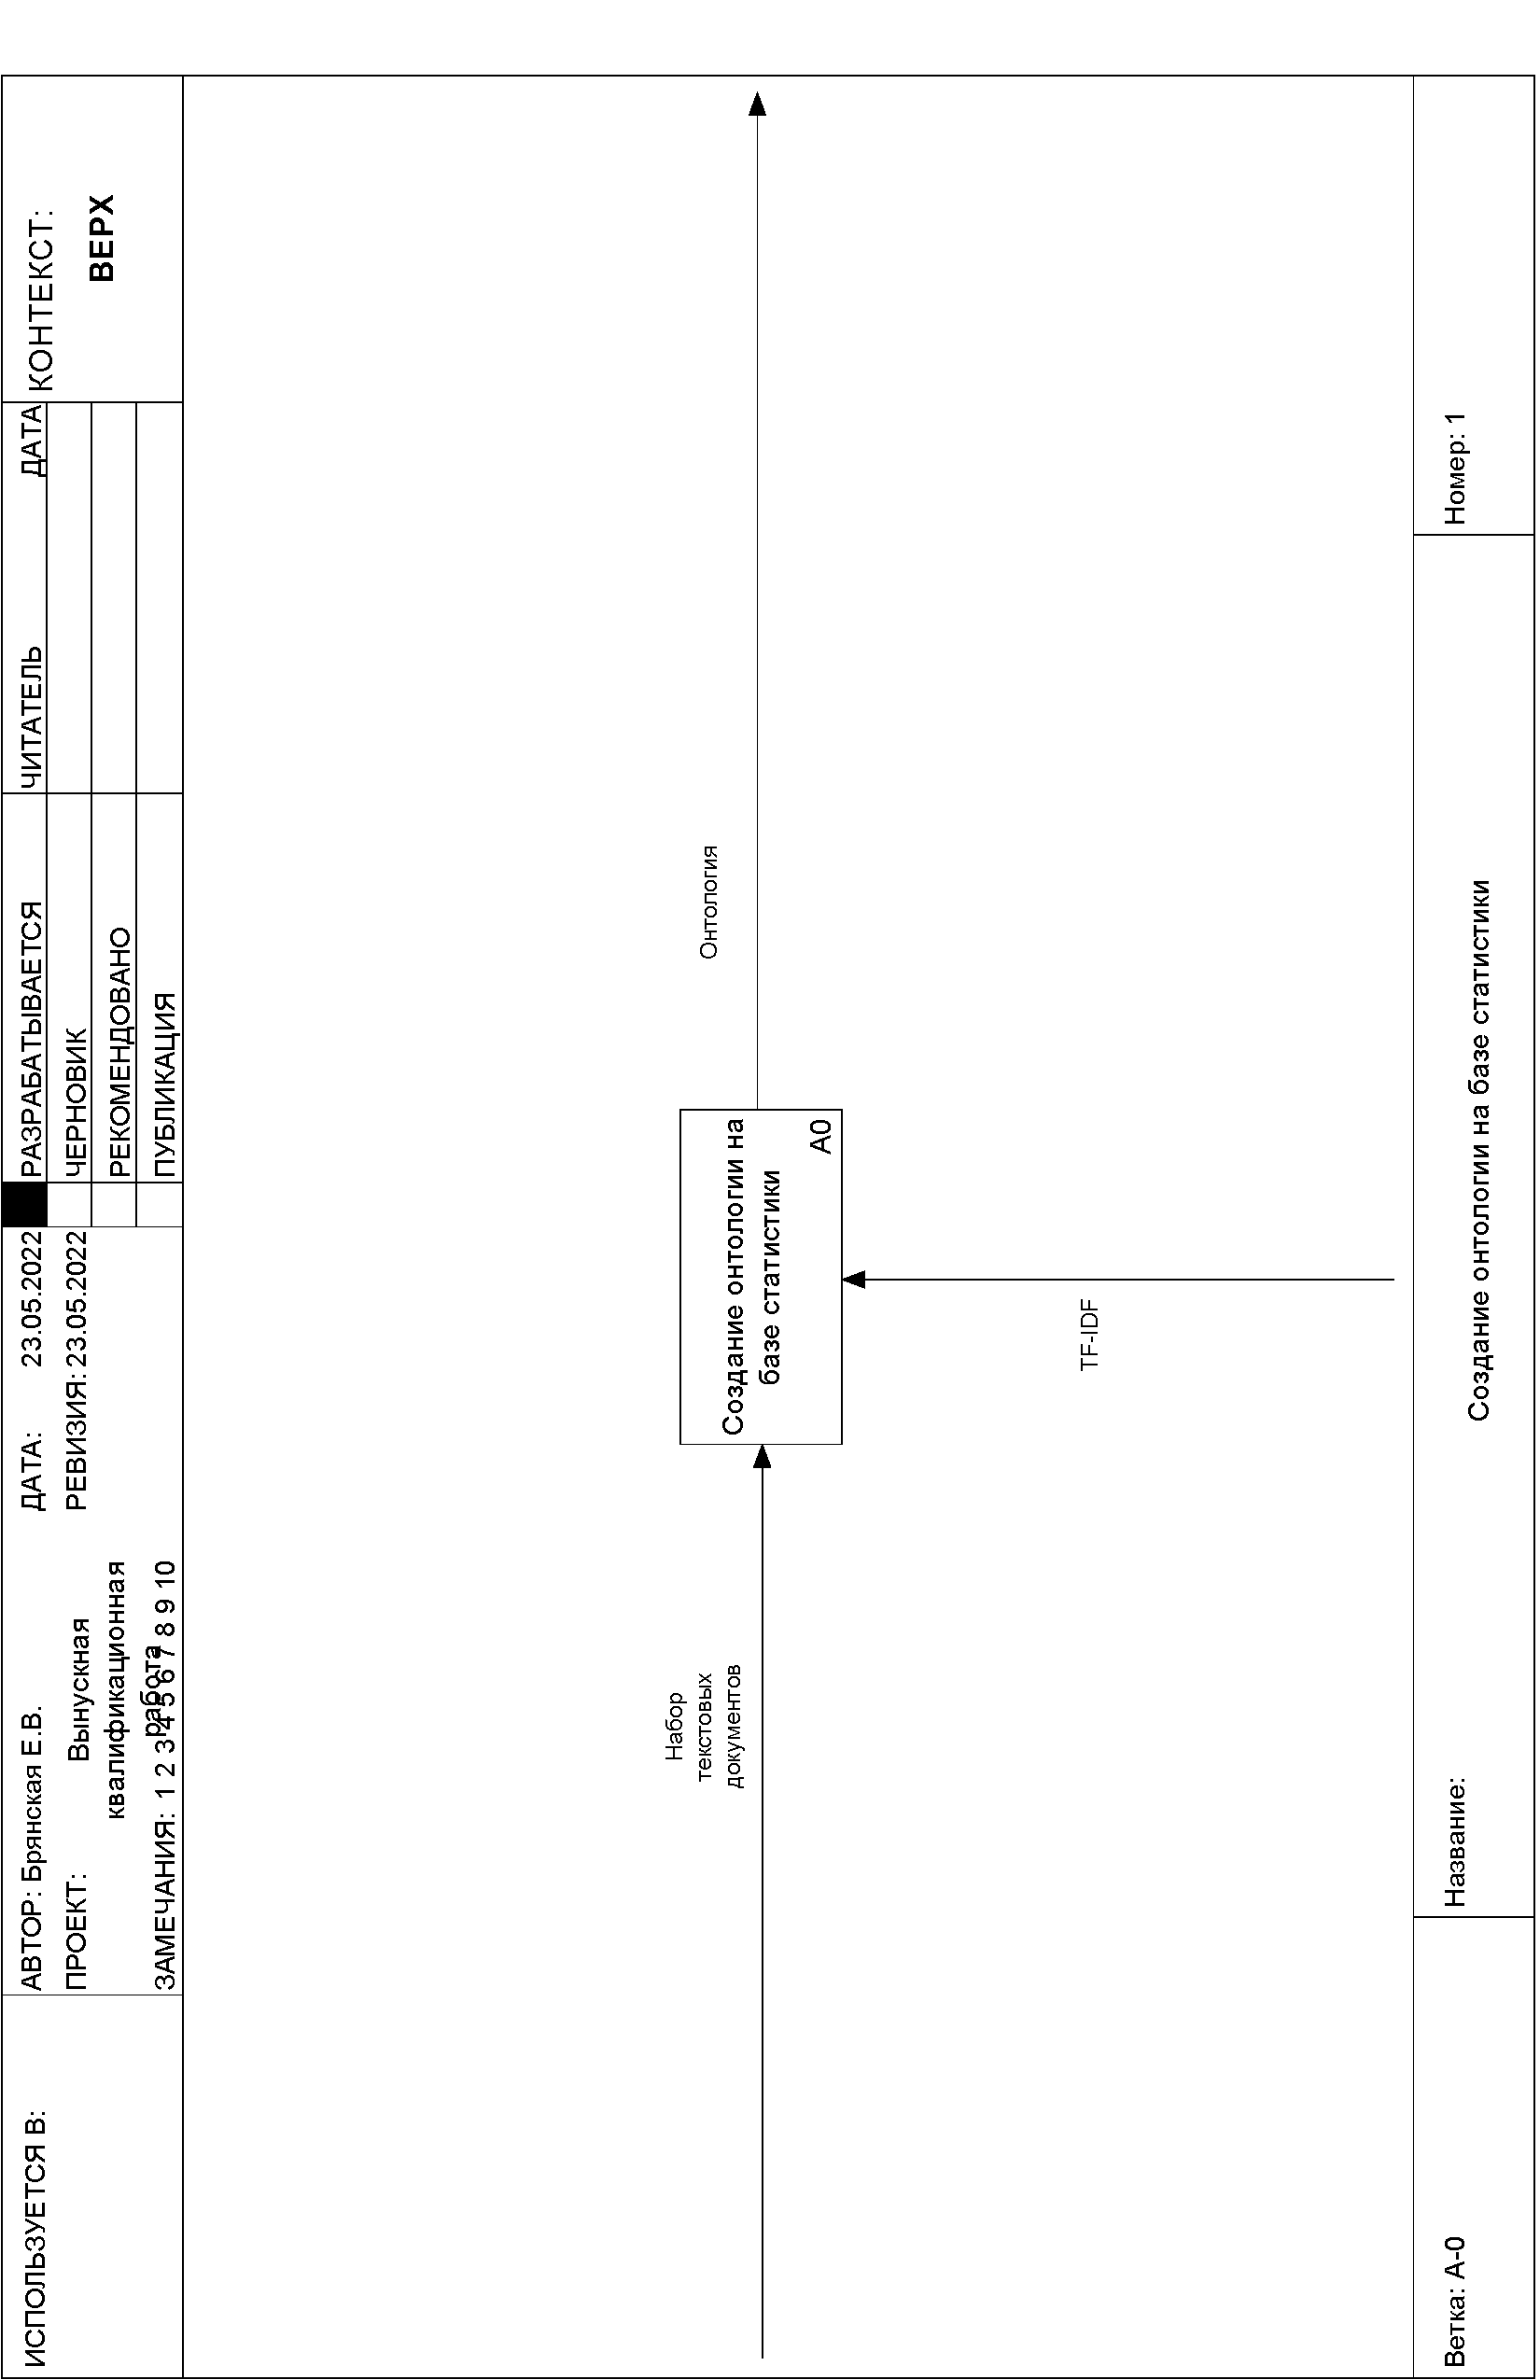
\includegraphics[scale = 0.39, angle=-90, page=1]{img/idef0/pdf/ontology.pdf}}
		\caption{Контекстная диаграмма метода создания онтологии на основе статистики.}
		\label{fig23:image}
	\end{center}
\end{figure}

\newpage

Сначала отбираются документы, содержащие определения одного термина, далее информация в каждом из них предобрабатывается, как описано в разделе \ref{sec:before_work}, и представляется в виде вектора.
\begin{figure}[h]
	\begin{center}
		{\includegraphics[scale = 0.39, angle=-90, page=2]{img/idef0/pdf/ontology.pdf}}
		\caption{Детализация метода создания онтологии на основе статистики.}
		\label{fig24:image}
	\end{center}
\end{figure}

\newpage

Шаги создания онтологии на основе синтаксических графов представлены на рисунках \ref{fig25:image}-\ref{fig27:image}.
\begin{figure}[h]
	\begin{center}
		{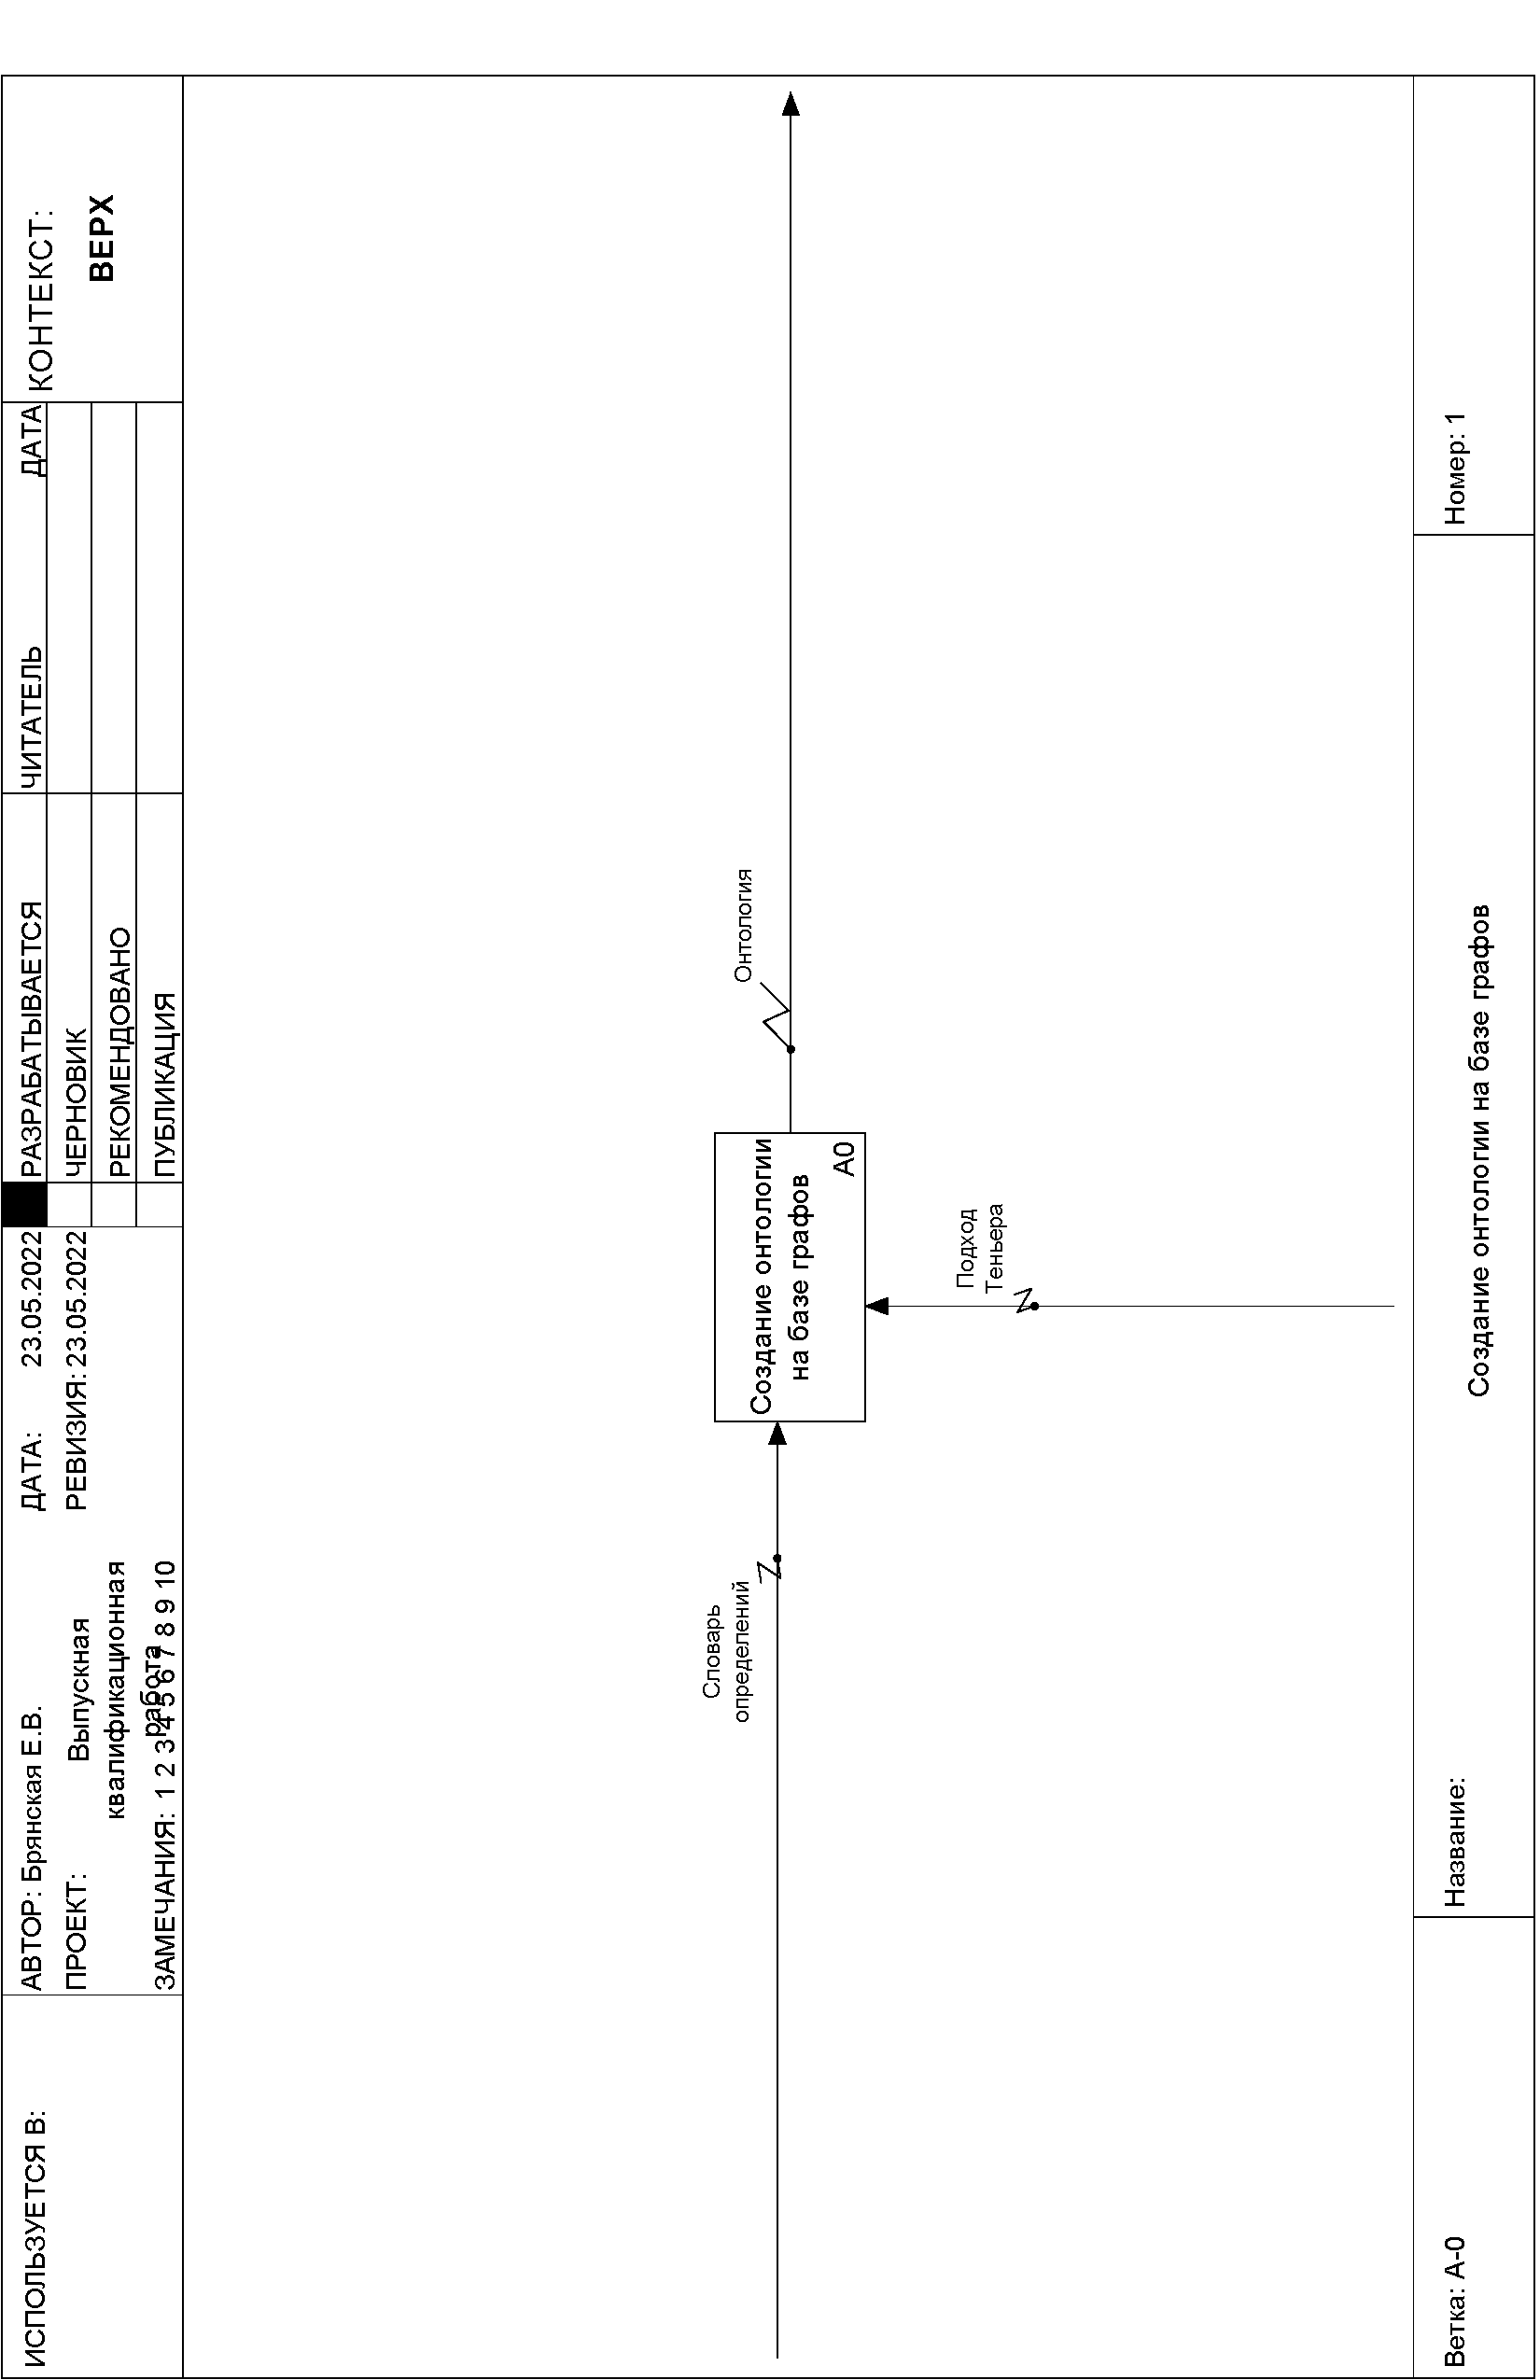
\includegraphics[scale = 0.39, angle=-90, page=1]{img/idef0/pdf/ontologyTree.pdf}}
		\caption{Контекстная диаграмма метода создания онтологии на основе графов.}
		\label{fig25:image}
	\end{center}
\end{figure}

\newpage
Каждый термин онтологии описывается ровно одним предложением, и для каждого из них строится соответствующий граф. Для всех слов в предложении определяются постоянные и непостоянные признаки, в предложении выделяются словосочетания, и на основе полученных данных формируется граф, который и становится элементом онтологии.
\begin{figure}[h]
	\begin{center}
		{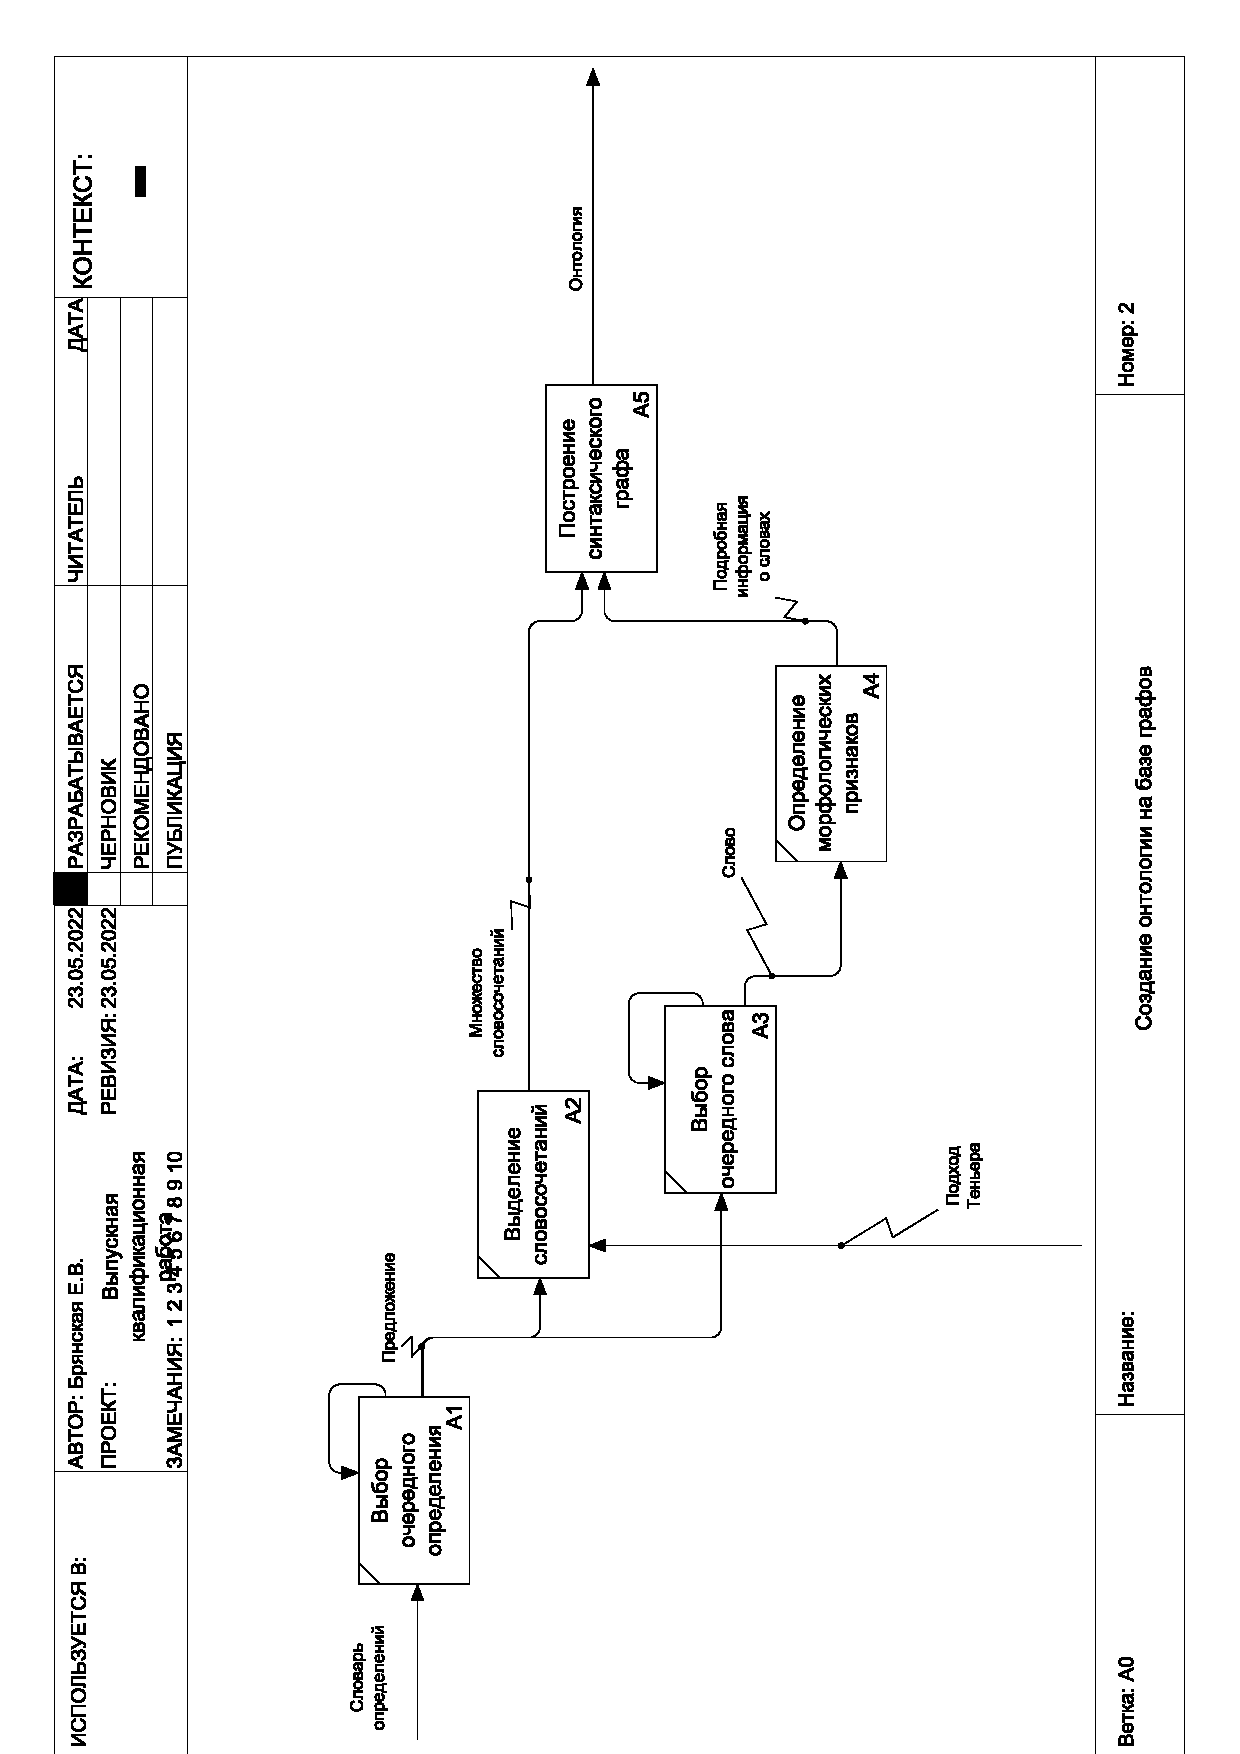
\includegraphics[scale = 0.57, angle=-90]{img/idef0/pdf/ontologyTree_2page.pdf}}
		\caption{Детализация метода создания онтологии на основе графов.}
		\label{fig26:image}
	\end{center}
\end{figure}

\newpage
Построение графа начинается с инициализации корня, затем последовательно обрабатывается каждое словосочетание и на основе полученной морфологической информации осуществляются дальнейшие действия: узел может быть добавлен или нет. 
\begin{figure}[h]
	\begin{center}
		{\includegraphics[scale = 0.39, angle=-90, page=3]{img/idef0/pdf/ontologyTree.pdf}}
		\caption{Декомпозиция блока А5.}
		\label{fig27:image}
	\end{center}
\end{figure}

\newpage

\subsection{Ключевые алгоритмы}
\subsubsection{Основной алгоритм}
Можно выделить следующие основные этапы:
\begin{enumerate}
	\item предобработка пользовательского ввода;
	\item выделение ключевых слов в запросе;
	\item поиск нечётких дубликатов, с использованием статистического метода;
	\item поиск нечётких дубликатов, с использованием сети из синтаксических графов (в случае не соответствия критерию принятия решения).
\end{enumerate}

Схема алгоритма приведена на рисунке \ref{fig33:image}. Все шаги более детально разобраны далее.
\begin{figure}[h]
	\begin{center}
		{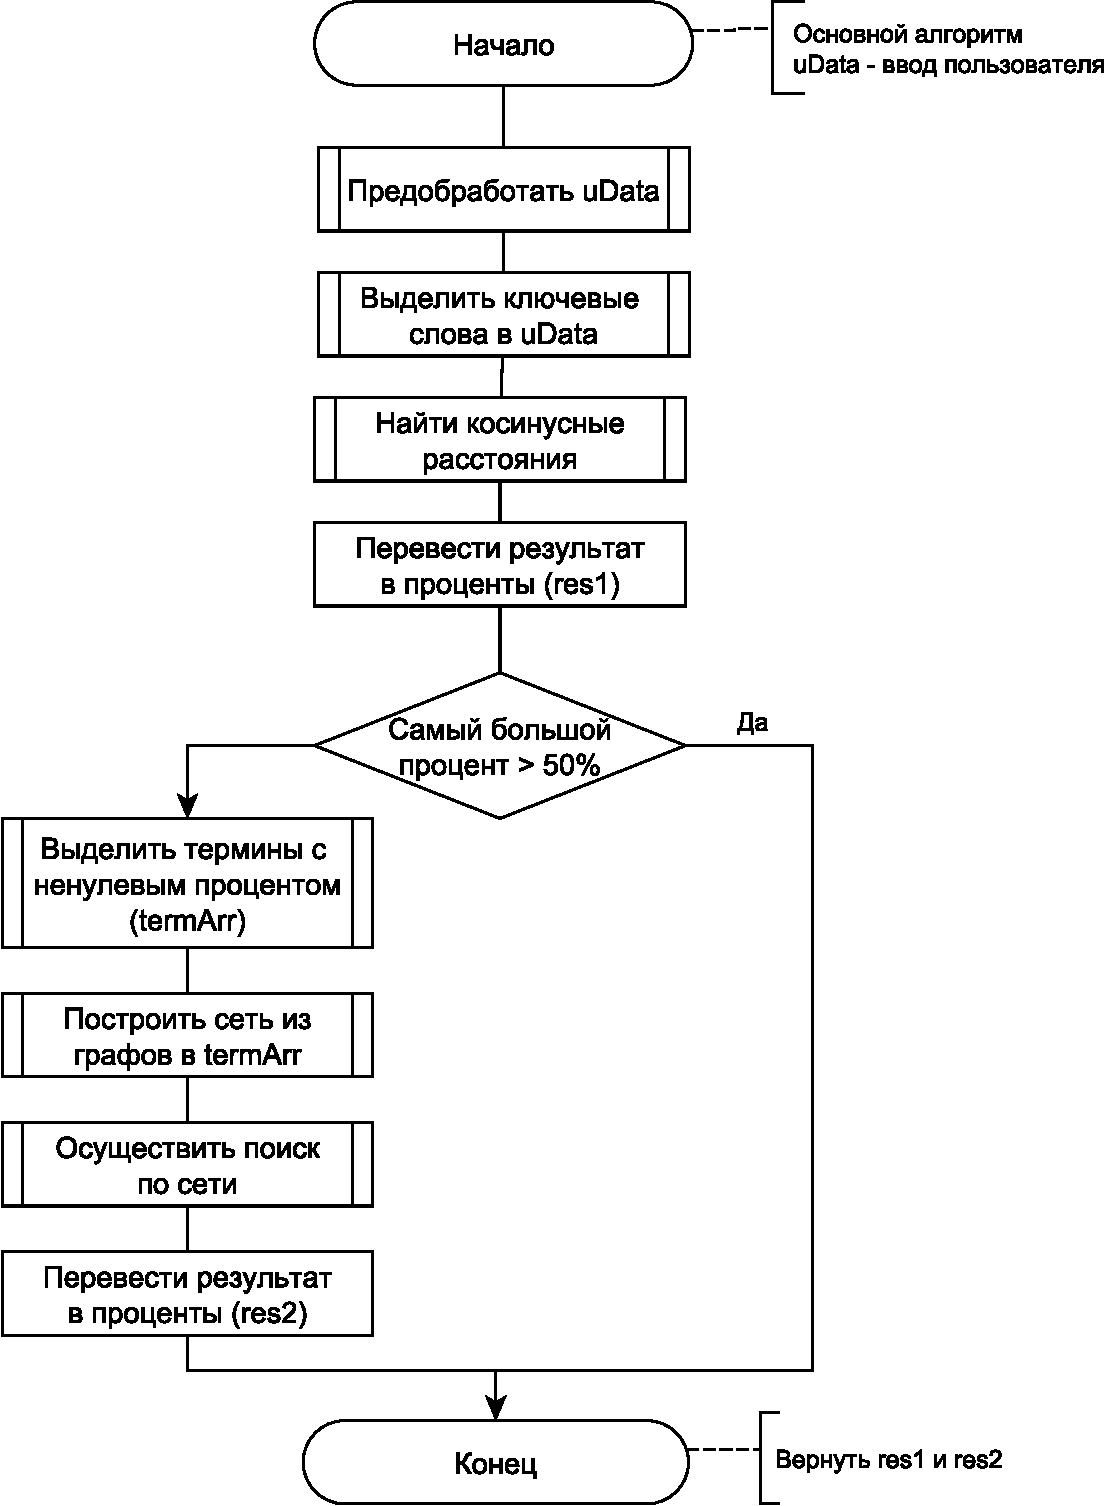
\includegraphics[scale = 0.6]{img/schemes/pdf/main.pdf}}
		\caption{Схема основного алгоритма.}
		\label{fig33:image}
	\end{center}
\end{figure}

\newpage

\subsubsection{Алгоритм предобработки данных}\label{sec:preprocess}
Предобработке подвергаются:
\begin{itemize}
	\item пользовательский ввод (в случае голосового ввода, он сначала переводится в текст, затем уже он подвергается обработке);
	\item текстовые данные для формирования онтологии на базе статистических данных;
	\item определения из словаря, предназначенные для создания синтаксических графов.
\end{itemize}

На рисунке \ref{fig28:image} представлена схема алгоритма обработки данных.

В процессе нормализации всё переводится в нижний регистр, удаляются все символы, кроме, букв русского языка, между словами выставляется фиксированно только один пробел.

Токенизация -- разделение на слова. На этапе лемматизации все слова приводятся к начальной форме, затем некоторые из них будут удалены, как стоп-слова. И для удобства распознавания терминов буква <<ё>> заменяется на <<е>>. 
\begin{figure}[h]
	\begin{center}
		{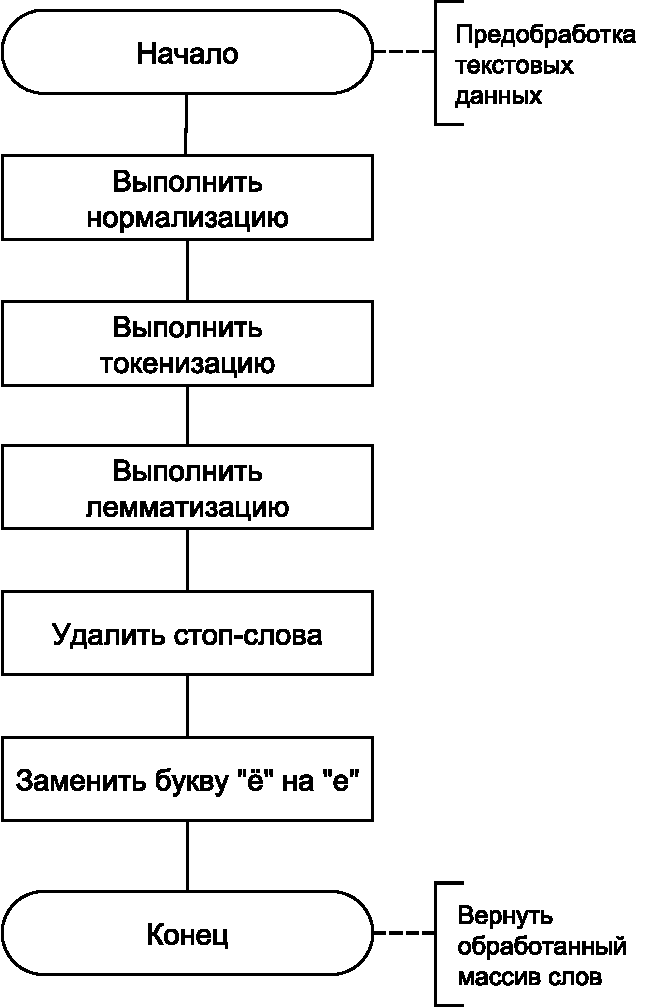
\includegraphics[scale = 0.6]{img/schemes/pdf/preprocess.pdf}}
		\caption{Схема алгоритма предобработки данных.}
		\label{fig28:image}
	\end{center}
\end{figure}

\subsubsection{Алгоритм создания онтологии на базе статистических данных}
На рисунке \ref{fig29:image} изображена схема алгоритма поиска ключевых слов. В основе лежит метод TF-IDF, описанный в разделе \ref{sec:weight}. 

Каждое описание проходит предобработку по алгоритму, который представлен в предыдущем разделе, далее для каждого слова подсчитывается число документов, в которых оно употреблено, и сколько раз. 

Затем вычисляется сам вес слова, как произведение этих величин, и в случае, если он удовлетворяет заранее заданным границам, то это слово считается ключевым для рассматриваемого термина. Подобные слова и формируют <<признаки>>, по которым в дальнейшем и будет проходить идентификация объекта.
\begin{figure}[h]
	\begin{center}
		{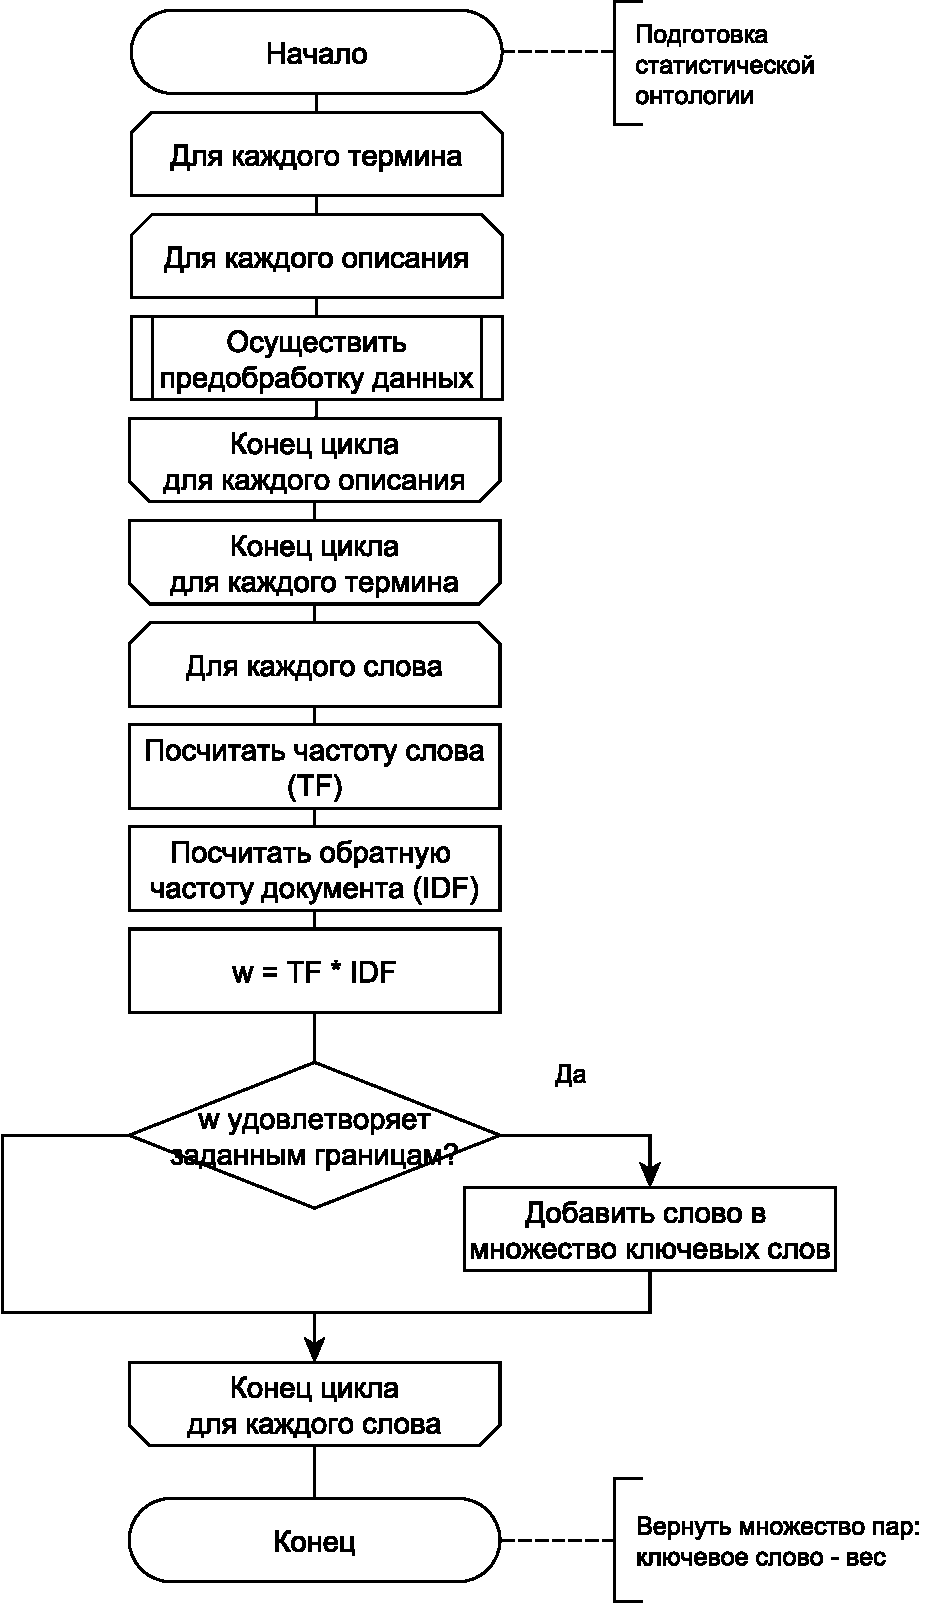
\includegraphics[scale = 0.6]{img/schemes/pdf/tf_idf.pdf}}
		\caption{Схема алгоритма создания онтологии с использованием статистического метода.}
		\label{fig29:image}
	\end{center}
\end{figure}

\subsubsection{Алгоритм создания онтологии на основе синтаксических графов}
Из-за того, что в большинстве инструментов для определения словосочетаний заложены принципы, которые определил Теньер, для решения поставленной задачи необходимо идентифицировать служебные части речи. 

В случае обнаружения и наличия зависимых от них слов, менять у детей этого элемента идентификатор родителя на идентификатор родителя для обрабатываемого слова. Таким образом, в синтаксическом дереве будут только слова, которые так или иначе несут смысловую нагрузку. 

На рисунке \ref{fig30:image} приведена подробная схема алгоритма.
\begin{figure}[h]
	\begin{center}
		{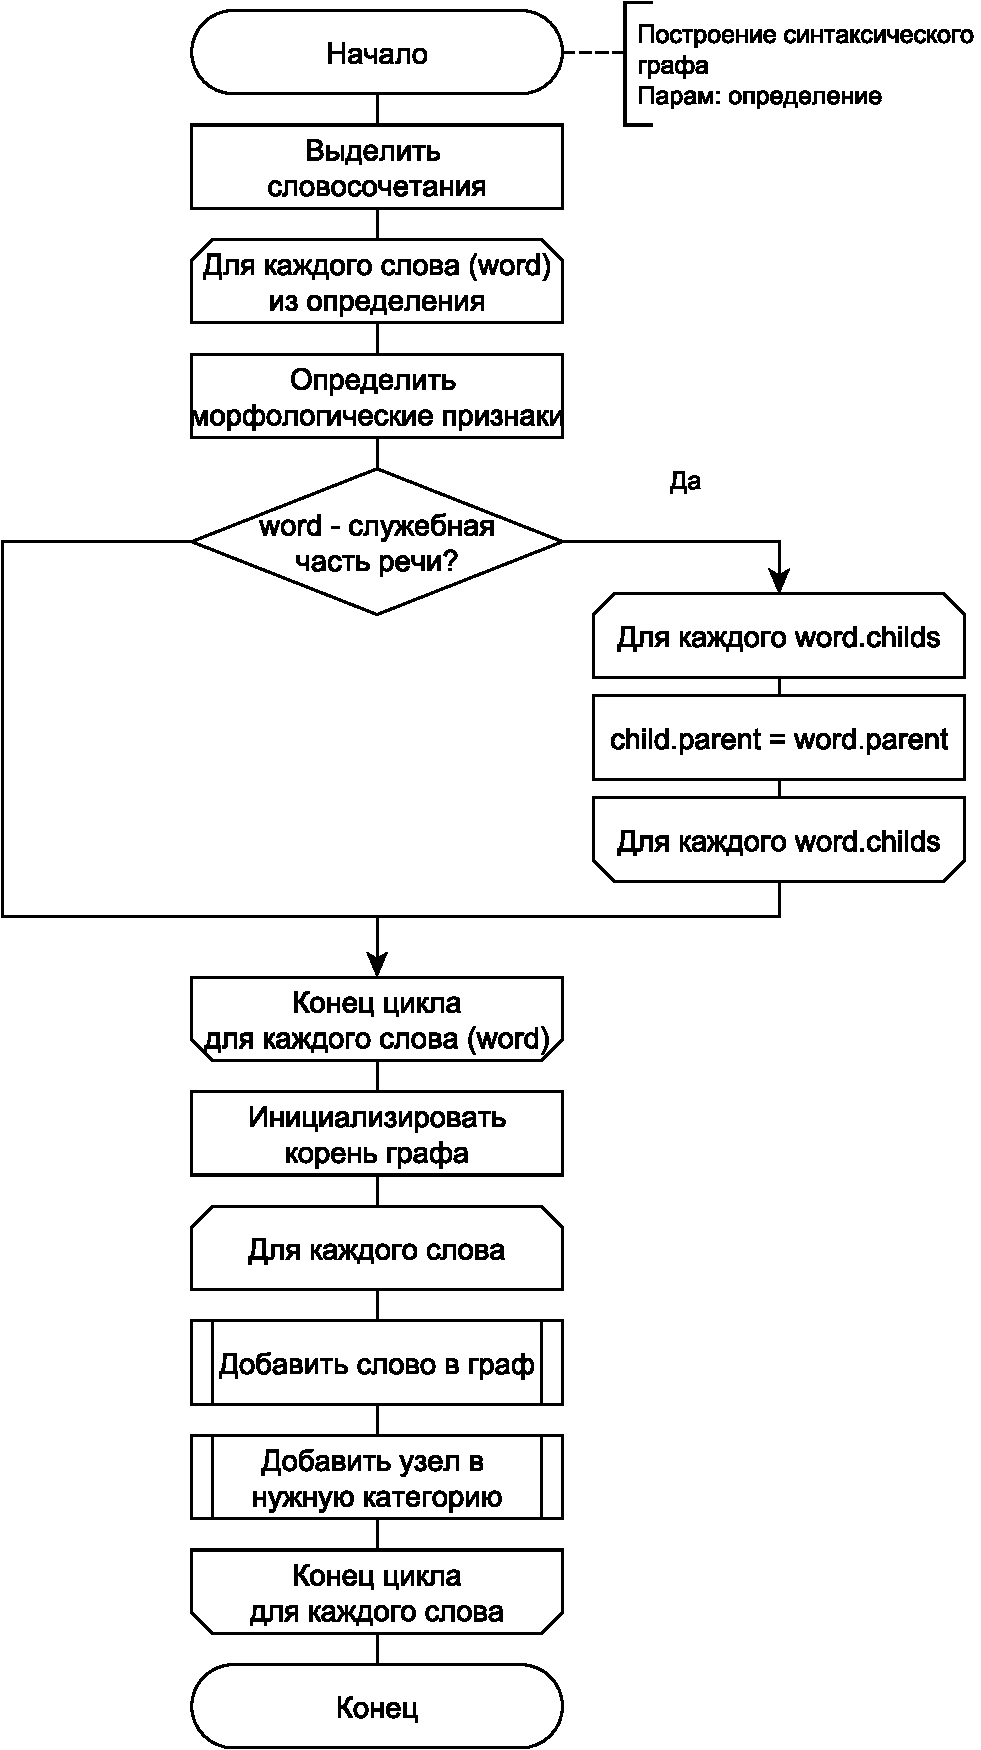
\includegraphics[scale = 0.6]{img/schemes/pdf/graph.pdf}}
		\caption{Схема алгоритма создания онтологии на основе графов.}
		\label{fig30:image}
	\end{center}
\end{figure}

\newpage

Само добавление узла в граф (рисунок \ref{fig31:image}) осуществляется только тогда, когда было установлено наличие родителя в графе. В противном случае создаётся <<пустой>> узел с идентификатором родителя. 

Если на момент добавления, в графе нет узла, ассоциированного с рассматриваемым словом, то добавляется новый узел. Если же узел есть, то он дополняется информацией (идентификаторы родителей, группы категорий и т.д.).
\begin{figure}[h]
	\begin{center}
		{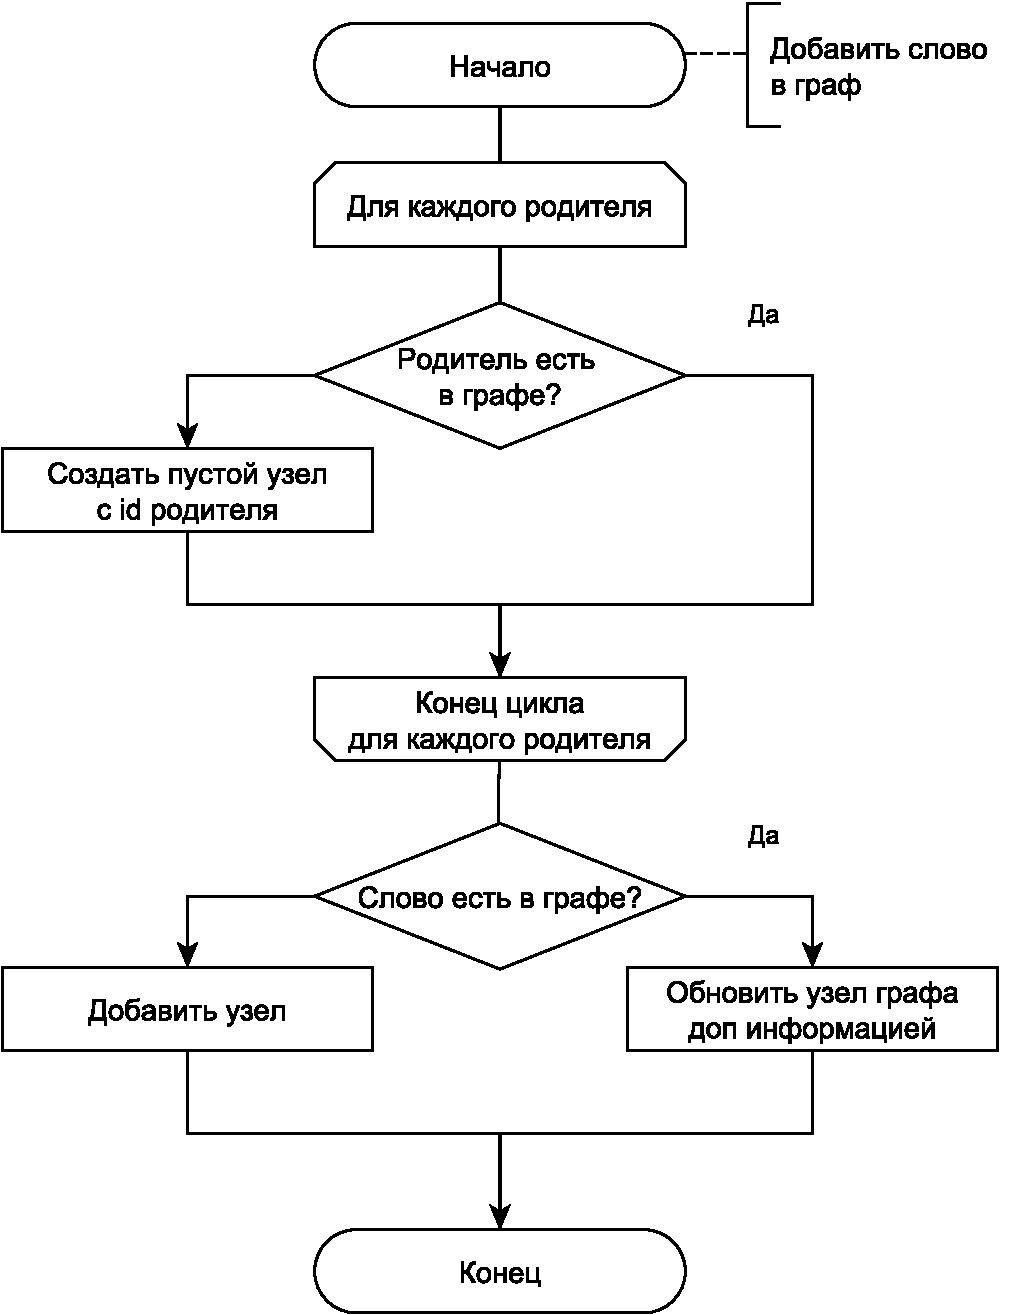
\includegraphics[scale = 0.6]{img/schemes/pdf/add_node.pdf}}
		\caption{Схема алгоритма добавления слова в граф.}
		\label{fig31:image}
	\end{center}
\end{figure}

Поскольку при идентификации объекта по его определению сначала просматриваются все объекты, связанные с термином, затем действия и т.д., то необходимо при формировании графа распределять детей каждого из узлов по категориям (рисунок \ref{fig32:image}). Это возможно благодаря заранее определённому постоянному морфологическому признаку -- часть речи.
\begin{figure}[h]
	\begin{center}
		{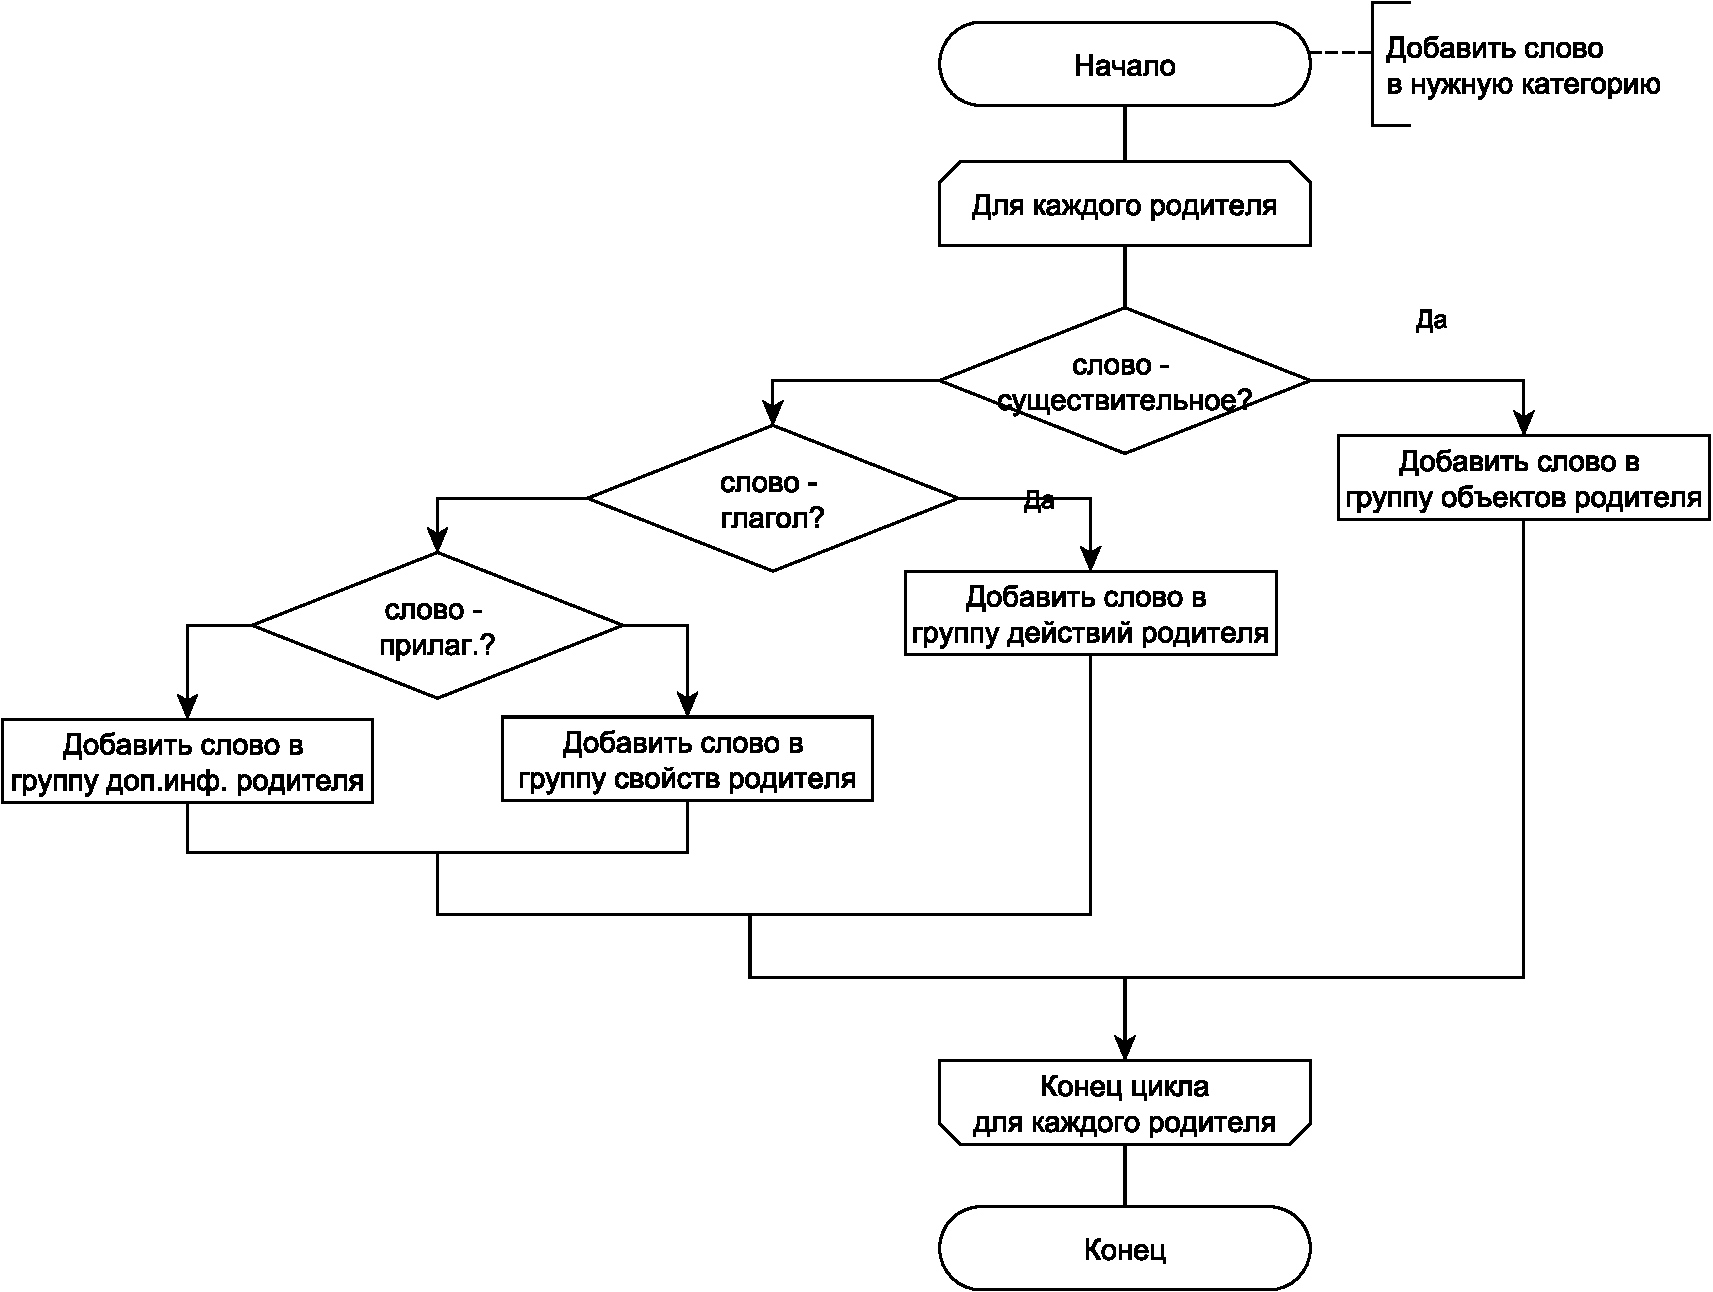
\includegraphics[scale = 0.58]{img/schemes/pdf/add_category.pdf}}
		\caption{Схема алгоритма добавления слова в нужную категорию.}
		\label{fig32:image}
	\end{center}
\end{figure}

\subsubsection{Алгоритм построения сети}
Сеть строится из синтаксических графов. При их слиянии необходимо следить за тем, чтобы не было дублирующих узлов (то есть, узлов, ассоциированных с одним и тем же словом). 

При обнаружении повторяющихся единиц, необходимо слить полезную информацию в уже существующий в графе узел.

На рисунке \ref{fig34:image} подробно изложен алгоритм построения сети.
\begin{figure}[h!]
	\begin{center}
		{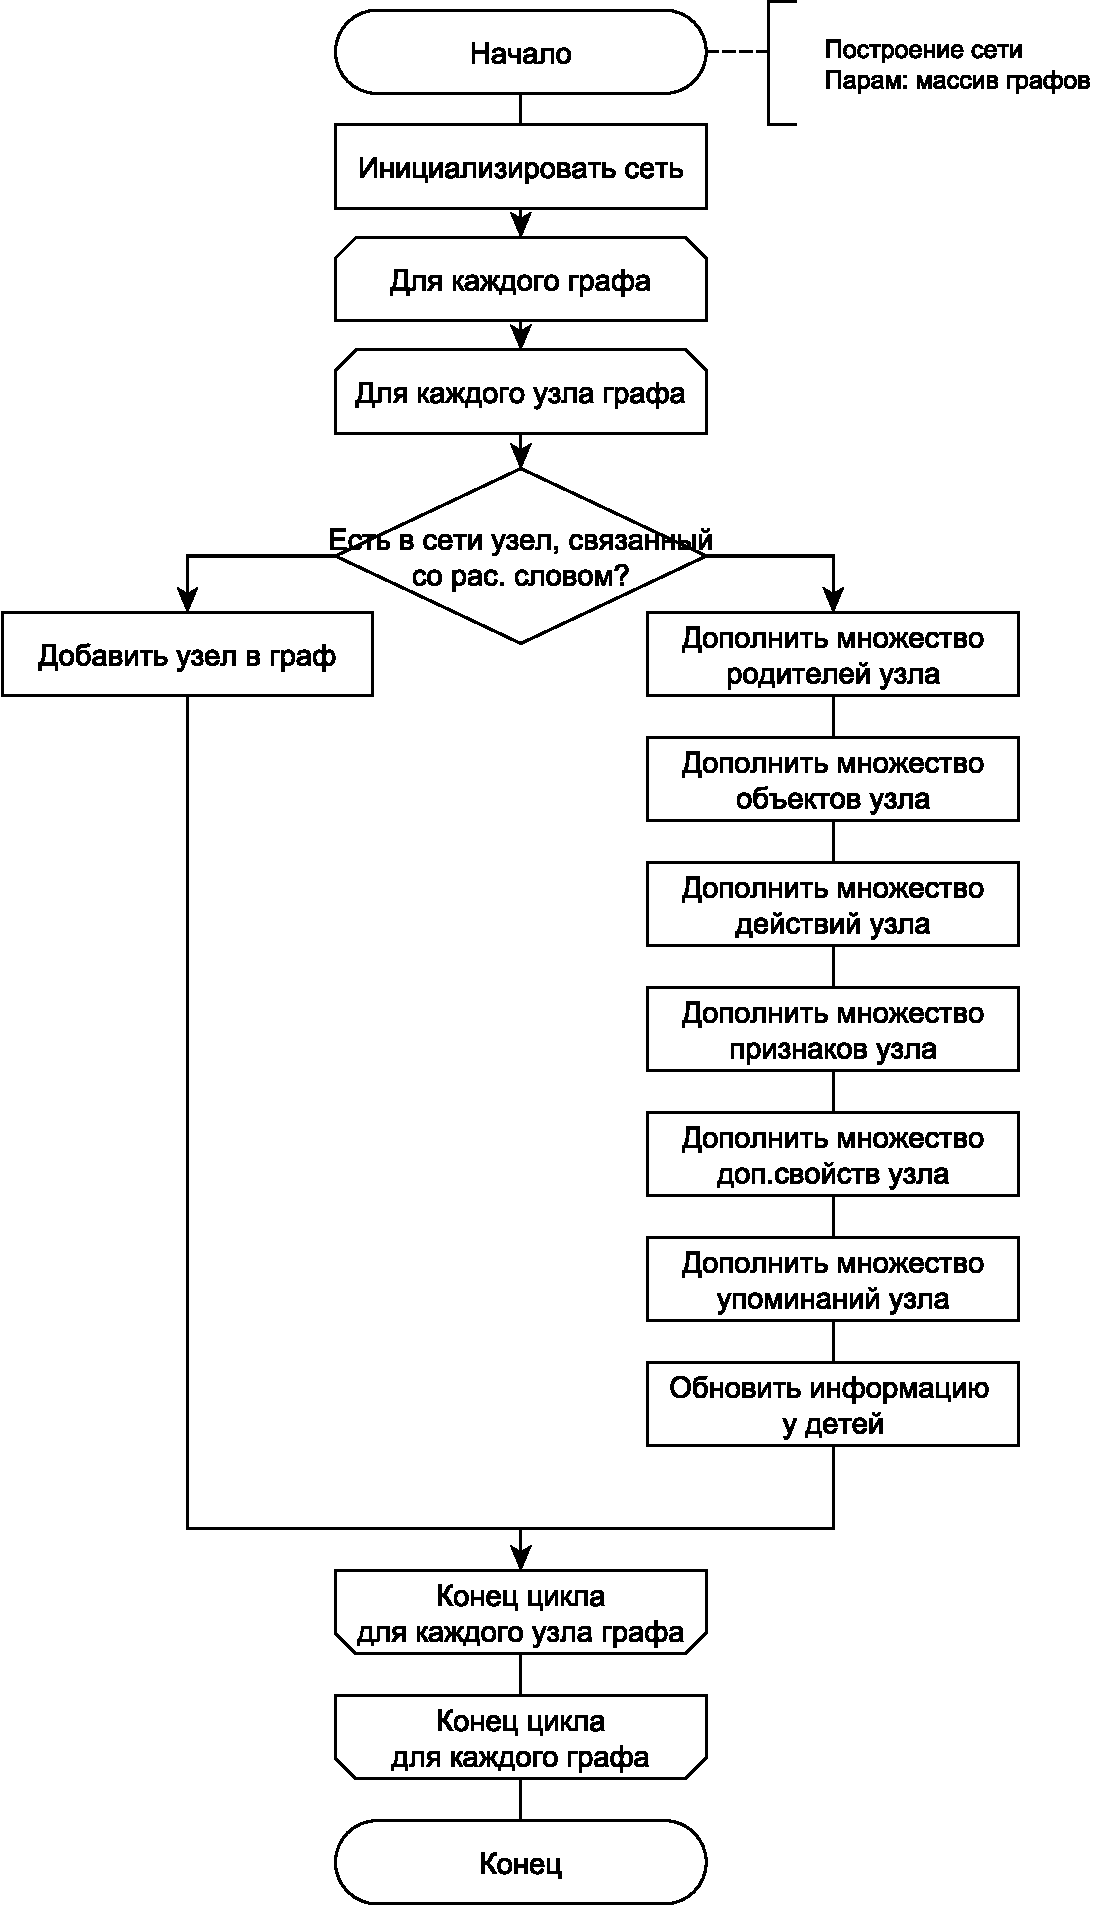
\includegraphics[scale = 0.6]{img/schemes/pdf/net.pdf}}
		\caption{Схема алгоритма построения сети.}
		\label{fig34:image}
	\end{center}
\end{figure}

\newpage

\subsubsection{Алгоритм поиска косинусного сходства}
Для того, чтобы найти нечёткие дубликаты, необходимо найти косинусное расстояние между тем, что ввёл пользователь, и заранее составленной онтологией.

На этом этапе привлекается формула \ref{formula6}. Каждое вычисленное значение сохраняется для дальнейшего принятия решения, какие термины наиболее подходят под описание пользователя.

На рисунке \ref{fig35:image} представлена схема алгоритма. Результатом его работы является массив косинусных расстояний. 

\begin{figure}[h]
	\begin{center}
		{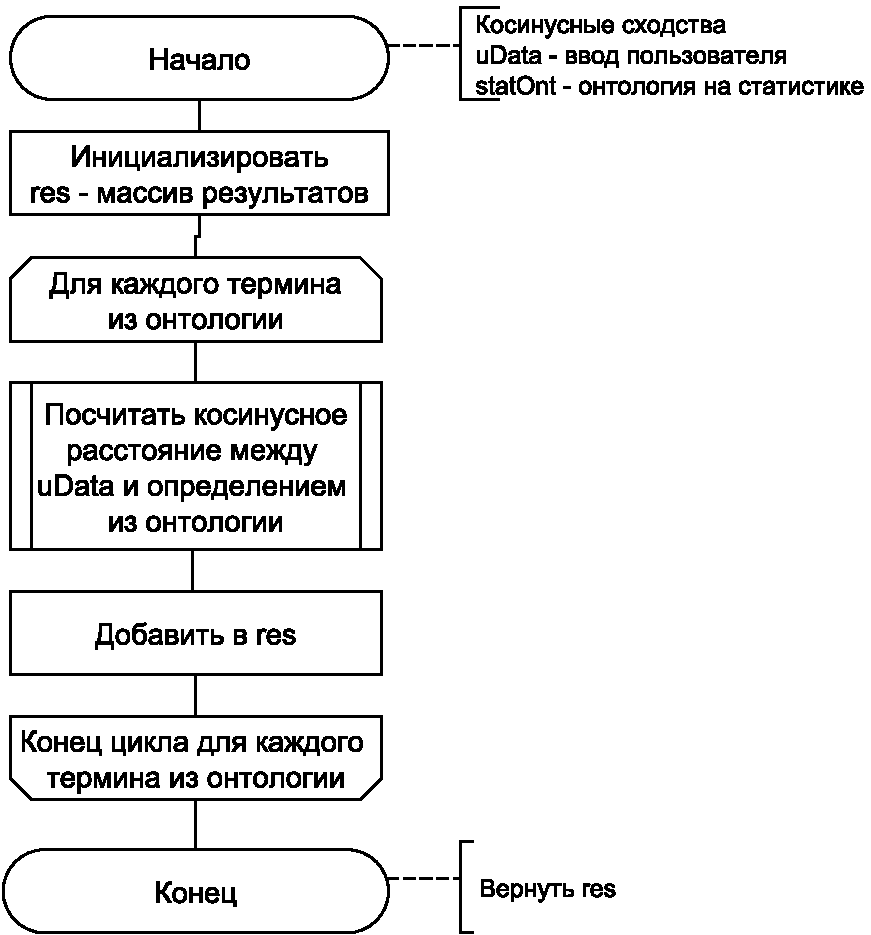
\includegraphics[scale = 0.6]{img/schemes/pdf/cos.pdf}}
		\caption{Схема алгоритма поиска косинусного сходства.}
		\label{fig35:image}
	\end{center}
\end{figure}

\subsubsection{Алгоритм поиска по сети}
В качестве структуры данных используется дек, который позволяет добавлять элементы как в <<голову>>, так и в <<хвост>>. 

По умолчанию сеть обходится в ширину (элемент снимается с головы, добавляется в хвост), причём каждое слово, связанное с обрабатываемым узел, проверяется на наличие в пользовательском вводе. Как только находится слово, присутствующее в обеих структурах, то потомки этого узла добавляются в голову дека (инициирование обхода в глубину) и увеличивается счётчик количества совпавших  слов.

Так происходит до тех пор, пока дек не опустеет. На рисунке \ref{fig36:image} подробно изложен этот алгоритм.
\begin{figure}[h!]
	\begin{center}
		{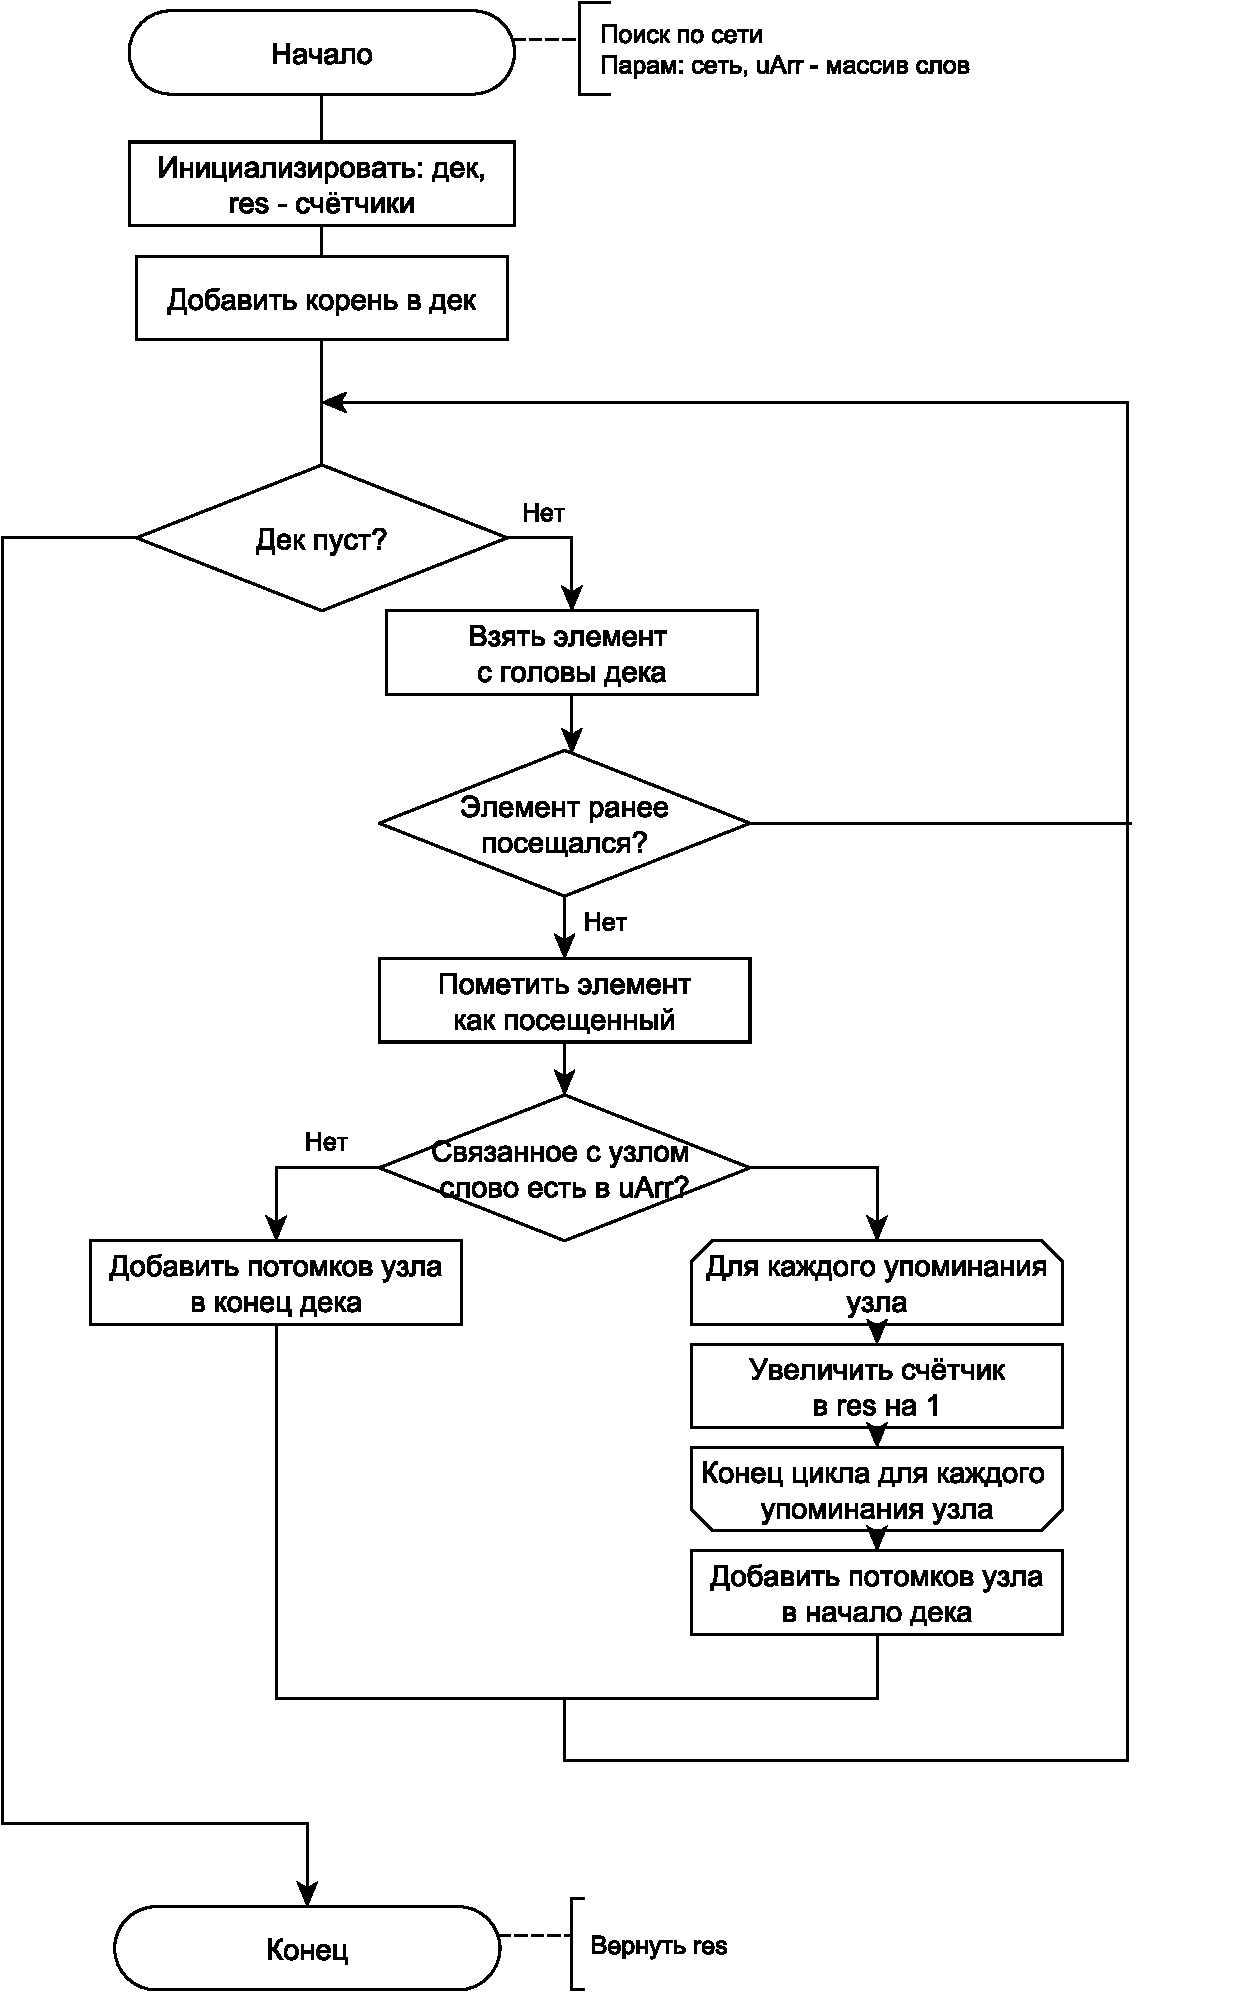
\includegraphics[scale = 0.6]{img/schemes/pdf/searchTree.pdf}}
		\caption{Схема алгоритма поиска по сети.}
		\label{fig36:image}
	\end{center}
\end{figure}

\newpage

\subsection{ER-диаграмма}
На рисунках \ref{fig37:image}-\ref{fig38:image} представлены ER-диаграммы для двух рассматриваемых онтологий. 

Сущность ключевого слова (Word) содержит такие поля, как название (name) и вес (weight). Из таких элементов состоит сущность Term (термин), в нём также хранится само название термина.
\begin{figure}[h]
	\begin{center}
		{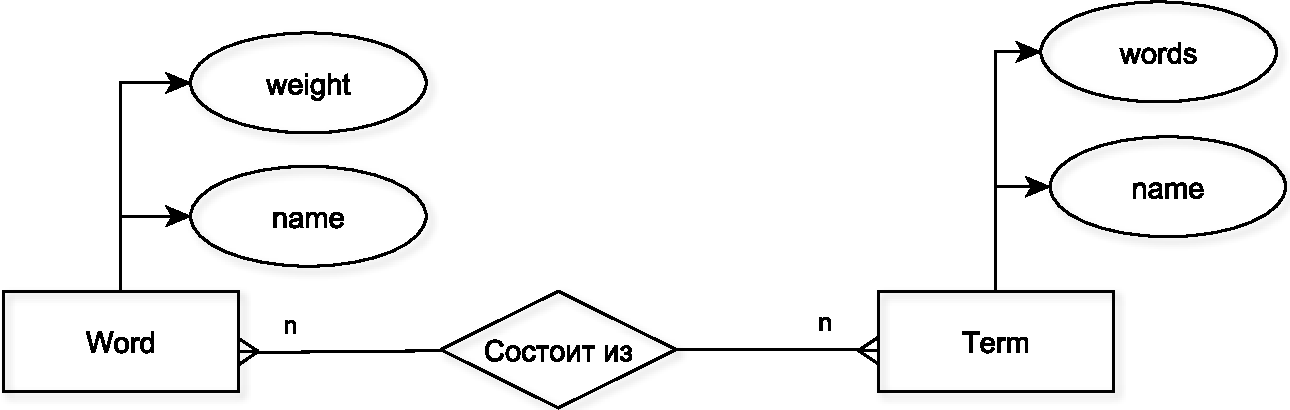
\includegraphics[scale = 0.6]{img/er/pdf/ontology.pdf}}
		\caption{ER-диаграмма сущностей статистической онтологии.}
		\label{fig37:image}
	\end{center}
\end{figure}

NodeTerm -- узел графа, который помимо названия объекта, с которым он связан, содержит информацию о его признаках, действиях, свойствах и т.д. Кроме того, хранится информация о терминах, в которых было употреблено данное слово (mentions). 

Согласно ранее установленным условиям, помимо того, что один граф может состоять из нескольких узлов, один узел может относиться к нескольким графам. 
Сущность сети включает как идентификационную информацию, так и информацию о её составляющих.

\begin{figure}[h]
	\begin{center}
		{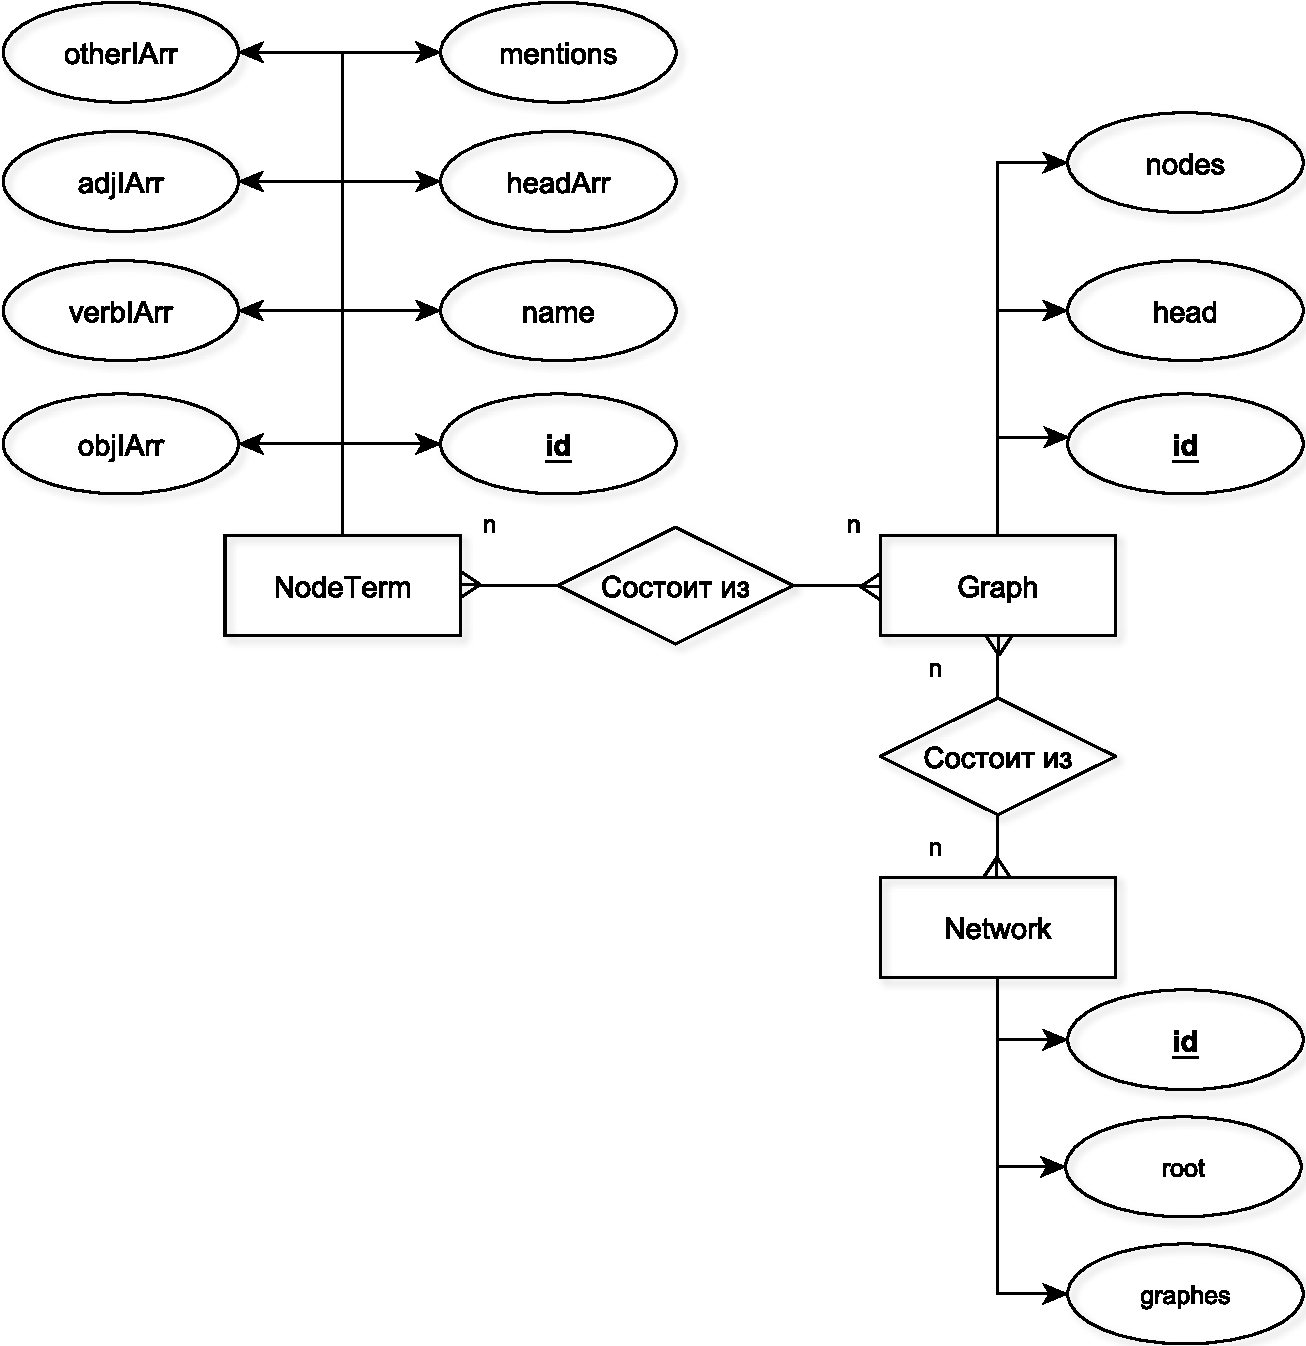
\includegraphics[scale = 0.6]{img/er/pdf/net.pdf}}
		\caption{ER-диаграмма сущностей онтологии на синтаксических графах.}
		\label{fig38:image}
	\end{center}
\end{figure}

\newpage

\subsection{Use-case диаграмма}
На рисунке \ref{fig39:image} продемонстрирована Use-case диаграмма, на которой наглядно показаны возможности каждого из участников. Выделяются две роли: пользователь и администратор. 

Для обоих предлагается два способа ввести запрос: через текстовое поле или через голосовой ввод. У обоих есть возможность просмотреть подробные результаты запроса  и локальную сеть запроса, если она была использована в методе.

Администратор, в отличие от пользователя, может вносить изменения в обе онтологии, и менять данные как по отдельным терминам, так и по всем сразу.

Дополнительно он может увидеть наглядное изображение всей сети и \, определения терминов из словаря.
\begin{figure}[h]
	\begin{center}
		{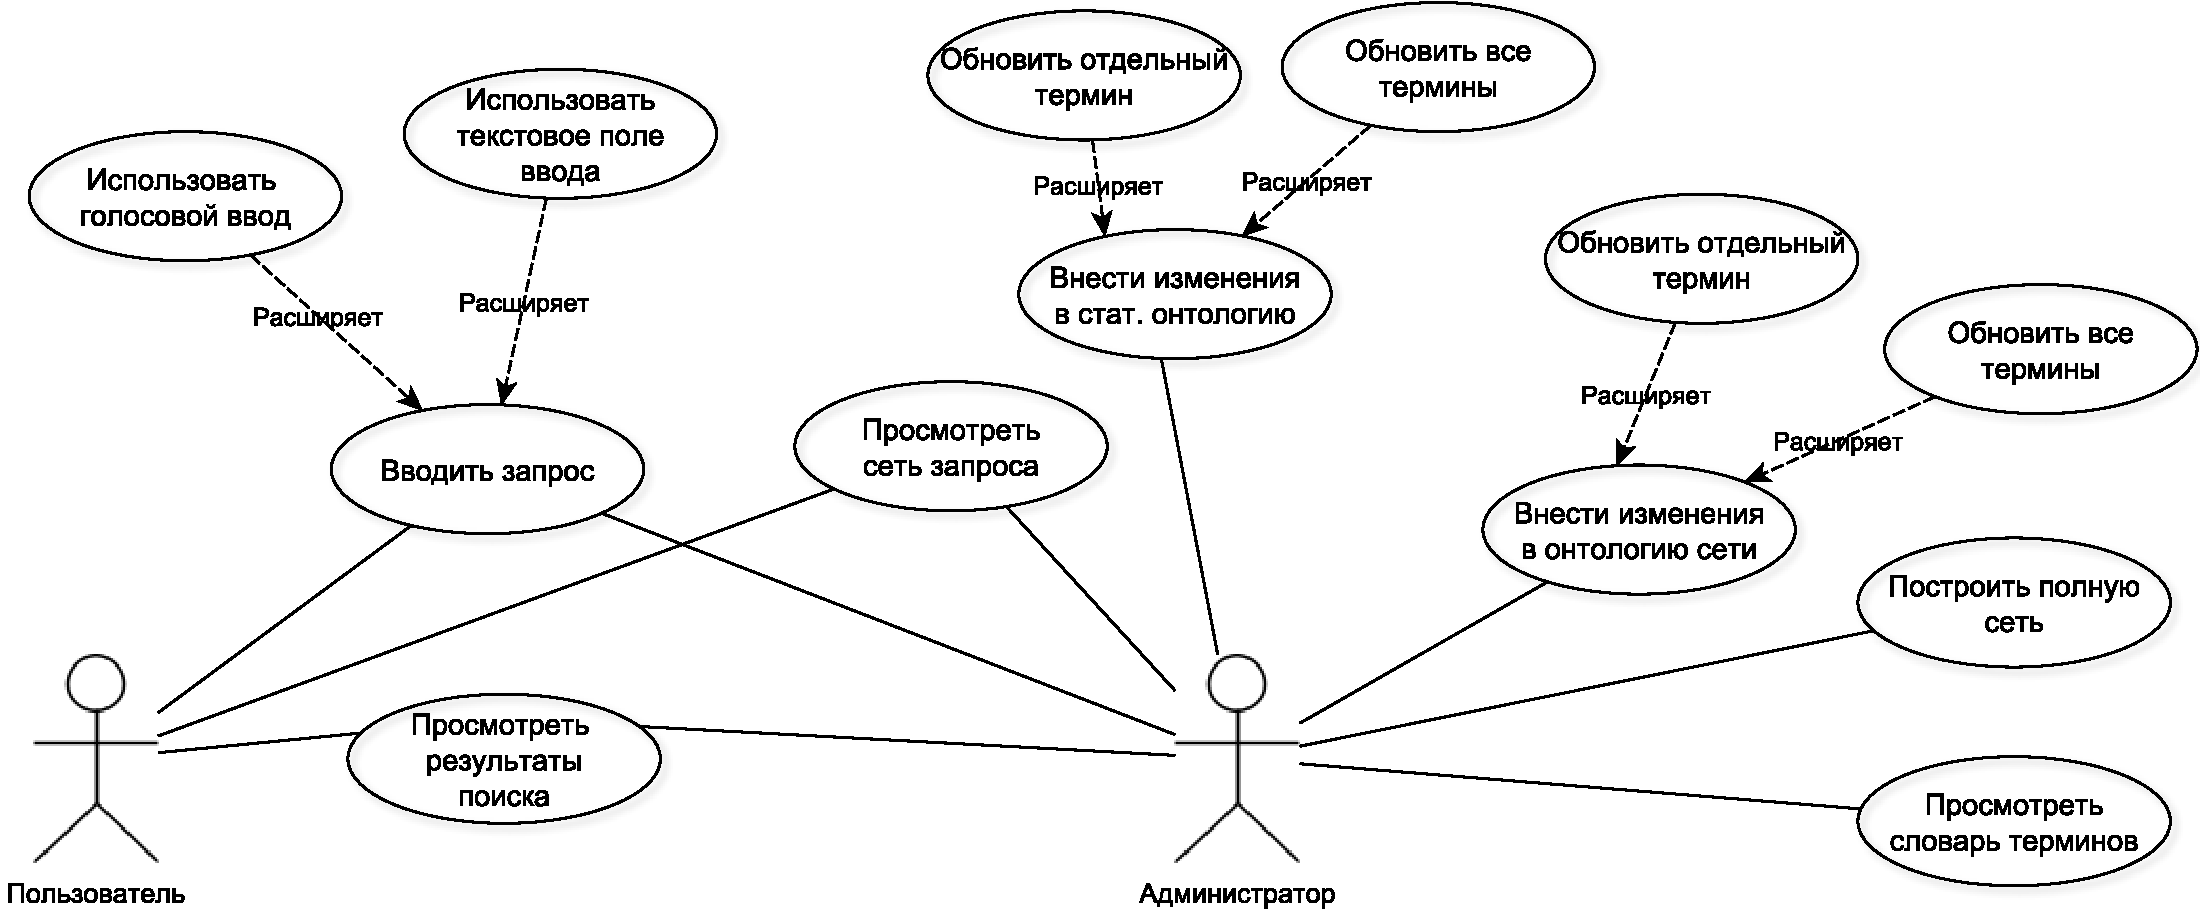
\includegraphics[scale = 0.45]{img/use_case/use_case.pdf}}
		\caption{Use-case диаграмма.}
		\label{fig39:image}
	\end{center}
\end{figure}

\subsection*{Выводы}
%\addcontentsline{toc}{subsection}{Выводы}
В текущем разделе был определён формат входных и выходных данных, предоставлены IDEF0 схемы, подробные схемы основных алгоритмов, use-case диаграмма.
